\pdfoutput=1

\documentclass{svjour3}                     % onecolumn (standard format)
%\documentclass[smallcondensed]{svjour3}     % onecolumn (ditto)
%\documentclass[smallextended]{svjour3}       % onecolumn (second format)
%\documentclass[twocolumn]{svjour3}          % twocolumn
%\usepackage[T1]{fontenc}


%\usepackage[displaymath]{lineno}

\smartqed  % flush right qed marks, e.g. at end of proof

\makeatletter
\renewcommand*{\@thmcounterend}{}
\makeatother
%\spnewtheorem{lemma}{Lemma}{\bfseries}{\itshape}
\spnewtheorem{assumption}{Assumption}{\bfseries}{\itshape}
%\spnewtheorem{remark}{Remark}{\bfseries}{\itshape}

%\usepackage{fullpage}
\usepackage{cite}
\usepackage[numbers,sort&compress]{natbib}

%\usepackage{slashbox} % for slashbox in tables

\usepackage{amsmath, amsfonts, amssymb}
\usepackage{stmaryrd} % for llbracket

%\newtheorem*{remark}{Remark}
%\theoremstyle{assumption}
%\newtheorem{assumption}{Assumption}
\usepackage{hyperref}
\hypersetup{colorlinks,
citecolor=blue
}

\usepackage[titletoc,toc,title]{appendix}
\usepackage{tikz}
%\usepackage{hhline}
\usepackage{graphicx, color, bm}
\usepackage{subfig}
\usepackage{pgfplots}
\usepackage{pgfplotstable}
\usepackage{slopetri} % my own package for drawing triangle slopes

\renewcommand{\hat}{\widehat}
\renewcommand{\tilde}{\widetilde}

%% d in integrand
\newcommand*\diff[1]{\mathop{}\!{\mathrm{d}#1}}
\newcommand{\diag}[1]{{\rm diag}\LRp{#1}}
\newcommand{\td}[2]{\frac{{\rm d}#1}{{\rm d}{\rm #2}}}
\newcommand{\pd}[2]{\frac{\partial#1}{\partial#2}}
\newcommand{\nor}[1]{\left\| #1 \right\|}
\newcommand{\LRp}[1]{\left( #1 \right)}
\newcommand{\LRs}[1]{\left[ #1 \right]}
\newcommand{\LRa}[1]{\left\langle #1 \right\rangle}
\newcommand{\LRb}[1]{\left| #1 \right|}
\newcommand{\LRc}[1]{\left\{ #1 \right\}}
\newcommand{\LRceil}[1]{\left\lceil #1 \right\rceil}
\newcommand{\LRl}[1]{\left. #1 \right|}
\newcommand{\pdn}[3]{\frac{\partial^{#3}#1}{\partial#2^{#3}}}
\newcommand{\Grad} {\ensuremath{\nabla}}
\newcommand{\jump}[1] {\ensuremath{\llbracket#1\rrbracket}}
\newcommand{\avg}[1] {\ensuremath{\LRc{\!\{#1\}\!}}}

\renewcommand{\note}[1]{{\color{blue}{#1}}}
\newcommand{\bnote}[1]{{\color{blue}{#1}}}
\newcommand{\rnote}[1]{{\color{red}{#1}}}

\graphicspath{{./figs/}}


%%%%%%%%%%%%%%%%%%%%%%%%%%%%%%%%%%%%%%%%%%%%%%%%%%%%%%%%%%%%%%%


%%%%%%%%%%%%%%%%%%%%%%%%%%%%%%%%%%%%%%%%%%%%%%%%%%%%%%%%%%%%%%%
%%%%%%%%%%%%%%%%%%%%%%%%%%%%%%%%%%%%%%%%%%%%%%%%%%%%%%%%%%%%%%%

\date{}
%\title{Skew-symmetric entropy stable modal discontinuous Galerkin formulations}% with applications to hybrid meshes}
%\titlerunning{Skew-symmetric entropy stable DG formulations}

\author{Jesse Chan, Mario Bencomo, David C.\ Del Rey Fernandez}
\title{Mortar-based entropy stable discontinuous Galerkin methods on non-conforming meshes}
\titlerunning{Mortar-based entropy stable DG methods}

\graphicspath{{./figs/}}

\begin{document}

\maketitle

\begin{abstract}
High order entropy stable discontinuous Galerkin (DG) methods for nonlinear conservation laws reproduce a discrete entropy inequality by combining entropy conservative finite volume fluxes with summation-by-parts (SBP) discretization matrices.  On tensor product (quadrilateral and hexahedral) elements, SBP matrices are typically constructed by collocating at Lobatto quadrature points.  Recent work has extended the construction of entropy stable DG schemes to collocation at more accurate Gauss quadrature points \cite{chan2018efficient}.  

In this work, we extend entropy stable Gauss collocation schemes to non-conforming meshes.  Entropy stable DG schemes require computing entropy conservative numerical fluxes between volume and surface quadrature nodes.  On conforming tensor product meshes where volume and surface nodes are aligned, flux evaluations are required only between ``lines'' of nodes.  However, on non-conforming meshes, volume and surface nodes are no longer aligned, resulting in a larger number of flux evaluations.  We reduce this expense by introducing an entropy stable mortar-based treatment of non-conforming interfaces via a face-local correction term, and provide truncation error estimates for the resulting discretizations.  Numerical experiments confirm the stability and accuracy of this approach, and we conclude by discussing how to extend mortar treatments of non-conforming interfaces to general elements and arbitrary quadrature rules \cite{chan2017discretely}.  
\end{abstract}



\section{Introduction}
Discretely entropy stability has emerged as a methodology for designing high order schemes for nonlinear conservation laws.  Entropy stable discretizations ensure the satisfaction of a semi-discrete entropy inequality by combining specific finite volume numerical fluxes with summation-by-parts (SBP) discretization matrices.  Compared to traditional high order methods, the resulting schemes demonstrate significantly improved robustness in the presence of under-resolved solution features such as shocks or turbulence while retaining high order accuracy.  

Entropy stable discontinuous Galerkin (DG) methods were originally constructed for quadrilateral and hexahedral meshes based on nodal collocation at Lobatto quadrature points \cite{fisher2013high, carpenter2014entropy, gassner2016split}.  Entropy stable schemes were later extended to simplicial and more general elements using tailored volume and surface quadrature rules \cite{chen2017entropy, crean2018entropy}.   More general quadrature rules were addressed in \cite{chan2017discretely, chan2018discretely, chan2018efficient, chan2019skew}, including entropy stable collocation schemes on quadrilateral and hexahedral elements based on more accurate Gauss quadrature rules and generalized SBP operators \cite{chan2018efficient}.

The work presented here focuses on geometrically non-conforming meshes.  Such meshes may arise when applying domain decomposition techniques to a complex geometry (e.g. meshing sub-domains independently)  \cite{bernardi1993domain} or performing local mesh refinement.  Entropy stable Lobatto collocation schemes have been constructed on non-conforming meshes in \cite{friedrich2017entropy} using SBP projection operators.  In this work, we extend entropy stable Gauss collocation to non-conforming quadrilateral and hexahedral meshes.  While it is straightforward to construct Gauss collocation schemes on non-conforming meshes, the treatment of non-conforming interfaces results in signficantly increased computational costs.  We reduce such costs by adopting a mortar-based treatment of non-conforming interfaces.  Moreover, while the cost of the proposed scheme is similar to that of  \cite{friedrich2017entropy} in 2D, the mortar-based approach is more computationally efficient for both Lobatto and Gauss collocation schemes on 3D non-conforming hexahedral meshes.  

The paper is organized as follows: Section~\ref{sec:0} briefly reviews the derivation of an entropy inequality for a system of nonlinear conservation laws.  Section~\ref{sec:1} introduces ``hybridized'' SBP operators as a unified way to treat both Lobatto and Gauss collocation schemes on conforming meshes of tensor product elements.  Section~\ref{sec:2} describes a naive extension to non-conforming meshes and illustrates why this formulation results in an increase in computational costs.  Section~\ref{sec:3} introduces a mortar-based formulation which addresses such costs, and characterizes the accuracy of the resulting formulations.  Section~\ref{sec:4} describes the extension to curved meshes, as well as more general elements and $p$ non-conformity.  We conclude with numerical validation of theoretical results in Section~\ref{sec:5}.  



\section{Entropy stability for systems of nonlinear conservation laws}
\label{sec:0}
We are interested in the numerical approximation of solutions to systems of nonlinear conservation laws
\begin{equation}
\pd{\bm{u}}{t} + \sum_{i=1}^d \pd{\bm{f}_i\LRp{\bm{u}}}{x_i} = 0.
\label{eq:nonlinpde}
\end{equation}
Here, $\bm{u}$ denotes the conservative variables and $\bm{f}_i(\bm{u})$ are nonlinear fluxes.  We briefly review entropy stability for systems of conservation laws in $d$ dimensions.  We assume there exists a convex scalar entropy $S(\bm{u})$ associated with (\ref{eq:nonlinpde}).  We then define the entropy variables $\bm{v}(\bm{u})$ as the gradient of the entropy $S(\bm{u})$ with respect to the conservative variables 
\[
\bm{v} = \pd{S(\bm{u})}{\bm{u}}.  
\]
For $S(\bm{u})$ convex, $\bm{v}(\bm{u})$ defines an invertible mapping between the conservative and entropy variables, whose inverse (from entropy to conservative variables) we denote by $\bm{u}(\bm{v})$.  Viscosity solutions to (\ref{eq:nonlinpde}) satisfy an integrated form of the entropy inequality \cite{dafermos2005compensated}
%\begin{gather}
%\pd{S(\bm{u})}{t} + \sum_{i=1}^d \pd{F_i(\bm{u})}{x_i} \leq 0, \qquad F_i(\bm{u}) = \bm{v}^T\pd{\bm{f}_i}{\bm{u}}, 
%\label{eq:entropyineq}
%\end{gather}
%Integrating (\ref{eq:entropyineq}) over a domain $\Omega$ and applying the divergence theorem yields 
\begin{equation}
\int_{\Omega} \pd{S(\bm{u})}{t} + \int_{\partial \Omega} \sum_{i=1}^d \bm{n}_i \LRp{\bm{v}^T\bm{f}_i(\bm{u}) - \psi_i(\bm{u})} \leq 0,
\label{eq:weakentropyineq}
\end{equation}
where $F_i$ denotes the $i$th scalar entropy flux function, $\psi_i(\bm{u}) = \bm{v}^T\bm{f}_i(\bm{u}) - F_i(\bm{u})$ denotes the $i$th entropy potential, $\partial \Omega$ denotes the boundary of $\Omega$ and $\bm{n}_i$ denotes the $i$th component of the outward normal on $\partial \Omega$.  This can be interpreted as implying that the time rate of change of entropy is bounded by the entropy flux through the boundary.



\section{Entropy stable collocation DG methods and hybridized SBP operators}
\label{sec:1}

In this section, we summarize the work of \cite{chan2018efficient} on the construction of entropy stable collocation DG methods based on generalized summation by parts (GSBP) operators.  These constructions are applicable to collocation schemes based on either Lobatto and Gauss nodes.  

\subsection{Hybridized SBP operators in 1D}

We begin by introducing collocation discretization matrices on the reference interval $[-1,1]$.  We assume the solution is collocated at $(N+1)$ quadrature points $x_i$ with associated quadrature weights $w_i$, and consider primarily Lobatto or Gauss quadrature points.  The collocation assumption is equivalent to approximating the solution using a degree $N$ Lagrange basis $\ell_j(x)$ at the $(N+1)$ quadrature points.  

We define mass and integrated differentiation matrices $\bm{M}, \bm{Q}$
\[
\bm{M}_{ij} = \int_{-1}^1 \ell_i(x)\ell_j(x), \qquad \bm{Q}_{ij} = \int_{-1}^1 \pd{\ell_j}{x}\ell_i.
\]
We assume that all integrals are computed using the collocated quadrature rule, such that 
\begin{gather*}
\bm{M}_{ij} = \int_{-1}^1 \ell_i(x)\ell_j(x) \approx \sum_{k=1}^{N+1} \ell_i(x_k)\ell_j(x_k) w_k = \delta_{ij} w_i\\
\bm{Q}_{ij} = \int_{-1}^1 \pd{\ell_j}{x}\ell_i \approx \sum_{k=1}^{N+1} \ell_i(x_k)\LRl{\pd{\ell_j}{x}}_{x_k} w_k.  
\end{gather*}
In other words, the mass matrix is diagonal with entries equal to the quadrature weights.  Since the integrands of $\bm{M}$ are degree $2N$ polynomials, the collocation approximation of $\bm{M}$ is exact for Gauss quadrature, but not for Lobatto quadrature.  For both Gauss and Lobatto quadrature, the matrix $\bm{Q}$ is exact under collocation quadrature.

We introduce the $2\times (N+1)$ matrix $\bm{E}$ which interpolates values at collocation nodes to values at the endpoints $x = -1$ and $x=1$.  These two matrices are defined entrywise as
\[
\LRp{\bm{E}}_{1i} = \ell_i(-1), \qquad  \LRp{\bm{E}}_{2i} = \ell_i(1).
\]
The mass and differentiation matrices satisfy a generalized summation by parts property \cite{fernandez2014generalized}
\begin{equation}
\bm{Q} = \bm{E}^T \bm{B} \bm{E} - \bm{Q}^T, \qquad \bm{B} = \begin{bmatrix}-1 & \\ & 1\end{bmatrix}.
\label{eq:gsbp}
\end{equation}
% The proof is a direct restatement of integration by parts, and can be found in \cite{fernandez2014generalized, ortleb2016kinetic, ortleb2017kinetic, ranocha2018generalised}.  
The GSBP property holds for both Lobatto and Gauss nodes, and switching between these two nodal sets simply requires redefining the matrices $\bm{D}, \bm{E}$.  For Gauss nodes, $\bm{E}$ is dense.  For Lobatto nodes, since the collocation nodes include boundary points, the interpolation matrix $\bm{E}$ reduces to the matrix which extracts nodal values associated with the left and right endpoints
\[
\bm{E} = \begin{bmatrix}
1 & 0 & \ldots & 0\\
0 & \ldots & 0 & 1
\end{bmatrix}.
\]

It is possible to construct energy stable high order discretizations of linear hyperbolic systems using GSBP operators based on Gauss nodes \cite{fernandez2014generalized}.  However, for nonlinear conservation laws, the presence of the dense $\bm{E}$ matrix in the GSBP property (\ref{eq:gsbp}) complicates the imposition of boundary conditions and computation of inter-element numerical fluxes \cite{crean2018entropy, chan2017discretely, chan2018efficient}.  This can be avoided by using ``hybridized'' (or decoupled) SBP operators \cite{chan2017discretely, chenreview, chan2019skew}, which are defined as the block matrix 
\[
\bm{Q}_h = \frac{1}{2}\begin{bmatrix}
\bm{Q}-\bm{Q}^T & \bm{E}^T\bm{B}\\
-\bm{B}\bm{E} & \bm{B}
\end{bmatrix}.
\]
The hybridized SBP operator satisfies a block form of the SBP property
\begin{equation}
\bm{Q}_h + \bm{Q}_h^T = \bm{B}_h, \qquad \bm{B}_h =  \begin{bmatrix}
\bm{0} & \\
& \bm{B}\end{bmatrix}.
\label{eq:hsbp}
\end{equation}
where $\bm{E}$ does not appear in the block boundary matrix on the right hand side.  Here, we have used $\bm{0}, \bm{1}$ to denote a matrix or vector of zeros or ones, where the size is inferred from context.  Note that the matrix $\bm{Q}_h$ also satisfies
\begin{equation}
\bm{Q}_h\bm{1} = 
\frac{1}{2}\begin{bmatrix}
\bm{Q}\bm{1}-\bm{Q}^T\bm{1} + \bm{E}^T\bm{B}\bm{1}\\
-\bm{B}\bm{E}\bm{1} - \bm{B}\bm{1}
\end{bmatrix}= 
\frac{1}{2}\begin{bmatrix}
\LRp{-\bm{Q}^T + \bm{E}^T\bm{B}}\bm{1}\\
\bm{0}
\end{bmatrix}=
\frac{1}{2}\begin{bmatrix}
\bm{Q}\bm{1}\\
\bm{0}
\end{bmatrix} = \bm{0}
\label{eq:Qh1}
\end{equation}
where we have used that $\bm{E}\bm{1} = \bm{1}$ (since $\bm{E}$ is a high order accurate boundary interpolation matrix), $\bm{Q}\bm{1} = \bm{0}$ (since $\bm{Q}$ is a differentiation matrix), and the GSBP property $-\bm{Q}^T + \bm{E}^T\bm{B}\bm{E} = \bm{Q}$

\subsection{Hybridized SBP operators in higher dimensions}

The formulation (\ref{eq:weakentropyineq}) can be extended to higher dimensions through a tensor product construction.  For simplicity, we illustrate this for 2D quadrilateral elements (the extension to 3D hexahedral elements is straightforward).  Let $\bm{M}_{\rm 1D}, \bm{Q}_{\rm 1D}$ denote one-dimensional generalized SBP norm (mass) and differentiation matrices, and let $\bm{E}_{\rm 1D}$ denote the 1D face interpolation matrix.  We define multi-dimensional  mass and differentiation matrices in terms of Kronecker products  
\begin{equation}
\hat{\bm{Q}}_1 = \bm{Q}_{\rm 1D} \otimes \bm{M}_{\rm 1D}, \qquad \hat{\bm{Q}}_2  = \bm{M}_{\rm 1D} \otimes \bm{Q}_{\rm 1D}, \qquad \hat{\bm{M}} = \bm{M}_{\rm 1D} \otimes  \bm{M}_{\rm 1D}.
\label{eq:kron}
\end{equation}
We also construct 2D face interpolation matrices from Kronecker products.  Let $\bm{E}_{\rm 1D}$ denote the one-dimensional face interpolation matrix, and let $\bm{B}_{\rm 1D}$ denote the 1D boundary matrix in (\ref{eq:gsbp}).  For a specific ordering of the face points, the two-dimensional face interpolation matrix $\bm{E}$ and reference boundary matrices $\hat{\bm{B}}_1, \hat{\bm{B}}_2$ are given by
\begin{equation}
\bm{E} = \begin{bmatrix}
\bm{E}_{\rm 1D} \otimes \bm{I}_{2}\\
\bm{I}_{2} \otimes \bm{E}_{\rm 1D} 
\end{bmatrix}, \qquad 
\hat{\bm{B}}_1 = \begin{bmatrix}
\bm{B}_{\rm 1D} \otimes \bm{M}_{\rm 1D} & \\
& \bm{0}
\end{bmatrix}, \qquad 
\hat{\bm{B}}_2 = \begin{bmatrix}
\bm{0} &\\
& \bm{M}_{\rm 1D} \otimes \bm{B}_{\rm 1D} 
\end{bmatrix},
\label{eq:EBdefs}
\end{equation}
where $\bm{I}_2$ is the $2\times 2$ identity matrix.  Recall that $\bm{M}_{\rm 1D}$ is the diagonal matrix of quadrature weights, so $\hat{\bm{B}}_i$ are diagonal.  

The construction of operators in (\ref{eq:kron}) and (\ref{eq:EBdefs}) correspond to the use of tensor product points quadrature points and \emph{aligned} surface points.  For example, if Gauss points are used for volume quadrature, we assume that Gauss points are also used for surface quadrature.  This ensures that the operators $\hat{\bm{Q}}_i, \hat{\bm{B}}_i, \bm{E}$ satisfy the analogous higher dimensional generalized SBP property $\hat{\bm{Q}}_i = \bm{E}^T\hat{\bm{B}}_i\bm{E} - \hat{\bm{Q}}_i^T$.

The 2D differentiation and interpolation matrices $\hat{\bm{Q}}_i, \bm{E}$ can now be used to construct 2D hybridized SBP operators.  Let $\hat{\bm{Q}}_{i,h}$ denote the hybridized SBP operator for the $i$th coordinate on the reference element, where $\hat{\bm{Q}}_{i,h}$ is defined as
\begin{align}
\hat{\bm{Q}}_{i,h} = \frac{1}{2}\begin{bmatrix}
\hat{\bm{Q}}_i - \hat{\bm{Q}}_i^T & \bm{E}^T\hat{\bm{B}}_i\\
-\hat{\bm{B}}_i\bm{E} & \hat{\bm{B}}_i
\end{bmatrix}.
\label{eq:hsbpdef}
\end{align}
These matrices satisfy the following multi-dimensional properties:
\begin{lemma}
\label{lemma:hsbprefprops}
Let $\hat{\bm{Q}}_{i}$ be defined as in (\ref{eq:kron}) and let $\hat{\bm{Q}}_{i,h}$ be defined as in (\ref{eq:hsbpdef}).  Then, 
\begin{align}
\hat{\bm{Q}}_{i,h} + \hat{\bm{Q}}_{i,h}^T = \begin{bmatrix}
\bm{0} & \\
& \hat{\bm{B}}_i
\end{bmatrix}, \qquad \hat{\bm{Q}}_{i,h}\bm{1} = \bm{0}.
\end{align}
\end{lemma}
The proof is contained in \cite{chan2018efficient}.  The SBP property follows from the construction of $\hat{\bm{Q}}_{i,h}$, and $\hat{\bm{Q}}_{i,h}\bm{1} = \bm{0}$ is a consequence of the Kronecker product and the same arguments used to derive (\ref{eq:Qh1}).  The construction of 3D differentiation and interpolation matrices proceeds similarly, and the matrices satisfy the same properties as described in Lemma~\ref{lemma:hsbprefprops}.  

%Then, a $d$-dimensional entropy conservative formulation on the reference element $[-1,1]^d$ is given as 
%\begin{gather}
%\hat{\bm{M}}\td{\bm{u}_h}{t} + \begin{bmatrix} \bm{I} \\ \bm{E} \end{bmatrix}^T
%\sum_{i=1}^d \LRp{2\hat{\bm{Q}}_{i,h} \circ \bm{F}_i}\bm{1} + \bm{E}^T\hat{\bm{B}}_i\LRp{\bm{f}_i^*-\bm{f}_i(\tilde{\bm{u}}_f)} = 0 \label{eq:esdgref}\\
%\LRp{\bm{F}_i}_{jk} = \bm{f}^i_S\LRp{\tilde{\bm{u}}_j,\tilde{\bm{u}}_k}
%\end{gather}
%where $\bm{f}^i_S$ is the numerical flux for the $i$th coordinate direction, and $\tilde{\bm{u}},\tilde{\bm{u}}_f$ are defined as in (\ref{eq:esdg1D}).  The proof is given in \cite{chan2017discretely, chan2018efficient}, and follows by applying the proof of Theorem~\ref{thm:esdg1D} to each coordinate direction.

%Finally, we can extend this formulation to the multi-element case.  
We now construct an entropy conservative formulation on an unstructured curved mesh.  
Suppose the domain $\Omega$ is decomposed into non-overlapping elements $D^k$ which are images of the reference mapping, such that $D^k$ is a differentiable mapping of the reference element $\hat{D} = [-1,1]^d$.  Let $\bm{x}_i$ denote the $i$th physical coordinate on $D^k$ and let $\hat{\bm{x}}_j$ denote the $j$th reference coordinate.  The mapping between reference and physical element induces scaled geometric terms 
\[
G_{ij} = J\pd{\hat{\bm{x}}_j}{\bm{x}_i},
\]
where $J$ denotes the determinant of the Jacobian of the physical-to-reference mapping.  We refer to $J$ as the Jacobian from here onwards.
These geometric terms also relate the normal vectors on reference and physical elements.  Let $\hat{\bm{n}}\hat{J}_f$ denote the outward normal vector on $\hat{D}$, scaled by the reference face Jacobians.  Then, the (scaled) physical normal vectors on $D^k$ are related to $\hat{\bm{n}}\hat{J}_f$ through
\begin{equation}
\bm{n}J_f = G\hat{\bm{n}}\hat{J}_f.
\label{eq:nJ_Gnhat}
\end{equation}
We assume that the mesh is watertight, such that the scaled normal vectors are equal and opposite across shared faces between two elements.  We also assume that the geometric terms ${G}_{ij}$ are constructed such that they are polynomials of degree less than or equal to $N$ and satisfy a discrete geometric conservation law (GCL)
\begin{equation}
\sum_{j=1}^d \pd{}{\hat{x}_j} G_{ij} = 0.
\label{eq:dgcl}
\end{equation}
The discrete GCL is satisfied automatically for isoparametric mappings in 2D, and there exist several techniques to enforce the satisfaction of a discrete GCL on various three-dimensional domains \cite{thomas1979geometric, kopriva2006metric, crean2018entropy, chan2018discretely, kozdon2018energy, kopriva2019free}.  

We can now assemble physical mass and differentiation matrices on $D^k$ from reference mass and differentiation matrices using the chain rule.  Let $\hat{\bm{Q}}_{j,h}$ denote the $j$th reference differentiation matrix on $\hat{D}$.  We can define the physical differentiation matrices $\bm{Q}_{i,h}$ on $D^k$ via the skew-symmetric splitting
\begin{equation}
\bm{Q}_{i,h} = \frac{1}{2}\sum_{j=1}^d \diag{\bm{G}_{ij}}\hat{\bm{Q}}_{j,h} + \hat{\bm{Q}}_{j,h} \diag{\bm{G}_{ij}},
\label{eq:curvedQ}
\end{equation}
where $\bm{G}_{ij}$ denotes the vector of values of $G_{ij} = J\pd{\hat{\bm{x}}_j}{\bm{x}_i}$ at both volume and surface points.  Since $G_{ij}$ is assumed to be a polynomial of degree less than or equal to $N$, $\bm{G}_{ij}$ is constructed using polynomial interpolation.

Because the reference matrices $\hat{\bm{Q}}_{j,h}$ satisfy the reference SBP properties (\ref{eq:hsbp}), one can show \cite{chan2018discretely} that the physical matrices $\bm{Q}_{i,h}$ satisfy analogous SBP properties.  
\begin{lemma}
\label{lemma:Qhprops}
Suppose the geometric terms $\bm{G}_{ij}$ satisfy the discrete GCL (\ref{eq:dgcl}), the normals are constructed via (\ref{eq:nJ_Gnhat}), and that $\bm{Q}_{i,h}$ is constructed using (\ref{eq:curvedQ}).  Then, 
\[
\bm{Q}_{i,h} + \bm{Q}_{i,h}^T = \begin{bmatrix}
\bm{0} &\\
& \bm{B}_i \end{bmatrix}, \qquad \bm{Q}_{i,h}\bm{1} = \bm{0},
\]
where $\bm{n}_i$ is a vector whose entries are values of the $i$th component of the scaled normals $n_iJ_f$ at face points, $\bm{w}_f$ is the vector of face quadrature weights $w_i$, and $\bm{B}_i = \diag{\bm{n}_i \circ \bm{w}_f}$.
\end{lemma}
\begin{proof}
The proof is identical to that of \cite{chan2018discretely}.  
We review it here for completeness.  Expanding out $\bm{Q}_{i,h} + \bm{Q}_{i,h}^T$ yields
\[
\frac{1}{2}\sum_{j=1}^d \diag{\bm{G}_{ij}}\hat{\bm{Q}}_{j,h} + \hat{\bm{Q}}_{j,h}^T\diag{\bm{G}_{ij}} + \hat{\bm{Q}}_{j,h} \diag{\bm{G}_{ij}} +  \diag{\bm{G}_{ij}}\hat{\bm{Q}}_{j,h}^T.
\]
For each term in the sum, we apply the SBP property of $\hat{\bm{Q}}_{j,h}$.  The volume terms cancel, leaving only surface terms
\[
\frac{1}{2}\sum_{j=1}^d \LRp{\hat{\bm{B}}_{j,h}\diag{\bm{G}_{ij}} +  \diag{\bm{G}_{ij}}\hat{\bm{B}}_{j,h}} = \begin{bmatrix}
\bm{0} &\\
& \bm{B}_i \end{bmatrix}.
\]
where we have used (\ref{eq:nJ_Gnhat}) and that $\hat{\bm{B}}_{j,h}$ and $\diag{\bm{G}_{ij}}$ are diagonal matrices.  

To show $\bm{Q}_{i,h}\bm{1} = \bm{0}$, we note that
\[
\bm{Q}_{i,h}\bm{1} = \frac{1}{2}\sum_{j=1}^d \diag{\bm{G}_{ij}}\hat{\bm{Q}}_{j,h}\bm{1} + \hat{\bm{Q}}_{j,h} \diag{\bm{G}_{ij}}\bm{1} = \frac{1}{2}\sum_{j=1}^d \hat{\bm{Q}}_{j,h} \bm{G}_{ij}
\]
since $\hat{\bm{Q}}_{j,h}\bm{1} = \bm{0}$ by Lemma~\ref{lemma:hsbprefprops}.  Note that, since $\bm{G}_{ij}$ is constructed using polynomial interpolation, $\bm{G}_{ij} = \LRs{G_{ij}(\hat{\bm{x}}), \quad \bm{E}G_{ij}(\hat{\bm{x}})}^T$, where $G_{ij}(\hat{\bm{x}})$ denotes the values of $G_{ij}$ at volume points.  The remaining term can be expanded out
\begin{align*}
\sum_{j=1}^d \hat{\bm{Q}}_{j,h} \bm{G}_{ij} &= \sum_{j=1}^d \begin{bmatrix} \hat{\bm{Q}}_jG_{ij}(\hat{\bm{x}}) - \hat{\bm{Q}}_j^TG_{ij}(\hat{\bm{x}}) + \bm{E}^T\bm{B}\bm{E}G_{ij}(\hat{\bm{x}})\\
\bm{B}\bm{E}G_{ij}(\hat{\bm{x}}) - \bm{B}\bm{E}G_{ij}(\hat{\bm{x}})
\end{bmatrix} \\
&=
\sum_{j=1}^d \begin{bmatrix} \LRp{- \hat{\bm{Q}}_j^T + \bm{E}^T\bm{B}\bm{E}}G_{ij}(\hat{\bm{x}})\\
\bm{0}
\end{bmatrix} = 
\sum_{j=1}^d \begin{bmatrix} \hat{\bm{Q}}_jG_{ij}(\hat{\bm{x}})\\
\bm{0}
\end{bmatrix}  = \bm{0},
\end{align*}
where we have used  the generalized SBP property and that $\sum_{j=1}^d\hat{\bm{Q}}_jG_{ij}(\hat{\bm{x}}) = \bm{0}$, since $G_{ij}$ satisfies the discrete GCL (\ref{eq:dgcl}), $G_{ij}(\hat{\bm{x}})$ is a polynomial of degree less than or equal to $N$, and $\hat{\bm{Q}}_j$ exactly differentiates polynomials of degree $N$.  
\qed\end{proof}

\subsection{Entropy conservative formulations on conforming meshes of mapped elements}

The aforementioned matrices can now be used to construct high order accurate entropy stable and entropy conservative schemes.  We first introduce an entropy conservative numerical flux \cite{tadmor1987numerical}.  Let $\bm{u}_L, \bm{u}_R$ denote left and right states in the conservative variables.  Then, an entropy conservative numerical flux is a vector-valued function $\bm{f}_{i,S}$ for $i = 1,\ldots,d$ which satisfies the following three properties
\begin{gather*}
\bm{f}_{i,S}\LRp{\bm{u},\bm{u}} = \bm{f}_i(\bm{u}), \qquad \text{(consistency)}\\
\bm{f}_{i,S}\LRp{\bm{u}_L,\bm{u}_R} = \bm{f}_{i,S}(\bm{u}_R,\bm{u}_L), \qquad \text{(symmetry)}\\
\LRp{\bm{v}_L-\bm{v}_R}^T\bm{f}_{i,S}\LRp{\bm{u}_L,\bm{u}_R} = \psi_i(\bm{u}_L) - \psi_i(\bm{u}_R), \qquad \text{(conservation)}.
\end{gather*}
Here, $\bm{v}_L, \bm{v}_R$ are the entropy variables evaluated at $\bm{u}_L, \bm{u}_R$, and $\psi_i$ is the $i$th entropy potential which appears in (\ref{eq:weakentropyineq}).  
Then, an entropy conservative scheme on a mapped element is given by
\begin{gather}
{\bm{M}}\td{\bm{u}_h}{t} + \begin{bmatrix} \bm{I} \\ \bm{E} \end{bmatrix}^T
\sum_{i=1}^d \LRp{2{\bm{Q}}_{i,h} \circ \bm{F}_i}\bm{1} + \bm{E}^T{\bm{B}}_i\LRp{\bm{f}_i^*-\bm{f}_i(\tilde{\bm{u}}_f)} = 0 \label{eq:esdg}\\
\LRp{\bm{F}_i}_{jk} = \bm{f}_S\LRp{\tilde{\bm{u}}_j,\tilde{\bm{u}}_k} \nonumber
\end{gather}
Here, the exterior state $\tilde{\bm{u}}_f$ used to evaluate the numerical flux $\bm{f}_i^*$ corresponds either to interface values on a neighboring element or an exterior state used to enforce boundary conditions, and $\circ$ denotes the matrix Hadamard product.  

%\note{Mention proof}
%Then, an entropy conservative scheme on the reference interval is given as
%\begin{gather}
%\bm{M}\td{\bm{u}_h}{t} + \begin{bmatrix} \bm{I} \\ \bm{E} \end{bmatrix}^T
%\LRp{2\bm{Q}_h \circ \bm{F}}\bm{1} + \bm{E}^T\bm{B}\LRp{\bm{f}^*-\bm{f}(\tilde{\bm{u}}_f)} = 0 \label{eq:esdg1D}\\ 
%\tilde{\bm{u}} = \begin{bmatrix}
%\bm{u}_h\\
%\tilde{\bm{u}}_f
%\end{bmatrix}, \qquad \tilde{\bm{u}}_f = \bm{u}\LRp{\bm{E}\bm{v}(\bm{u}_h)},\nonumber \\ 
%\LRp{\bm{F}}_{jk} = \bm{f}_S\LRp{\tilde{\bm{u}}_j,\tilde{\bm{u}}_k}, \qquad \bm{f}^* = \bm{f}_S\LRp{\tilde{\bm{u}}_f^+,\tilde{\bm{u}}_f}.\nonumber
%\end{gather}
%Here, $\tilde{\bm{u}}_f^+$ denotes some exterior state which can be used to enforce boundary conditions or coupling between different elements

\begin{theorem}
\label{thm:esdg}
Assuming continuity in time, the formulation (\ref{eq:esdg}) is entropy conservative in the sense that
\[
\bm{1}^T\bm{M}\td{S(\bm{u}_h)}{t} + \bm{1}^T\bm{B}_i\LRp{\bm{v}_f^T\bm{f}_i^* - \psi_i(\tilde{\bm{u}}_f)} = 0, \qquad \bm{v}_f =\bm{E}\bm{v}(\bm{u}_h).
\]
\end{theorem}
\begin{proof}
The proof uses similar techniques as proofs in other papers \cite{chen2017entropy, crean2018entropy, chan2017discretely, chan2019skew}, and we repeat it for completeness.  We begin by testing (\ref{eq:esdg}) with the vector of entropy variables evaluated at nodal points $\bm{v}(\bm{u}_h)$.  We apply the chain rule in time and use that $\bm{M}$ is diagonal to show that 
\[
\bm{v}(\bm{u}_h)^T\bm{M}\td{\bm{u}}{t} = \bm{1}^T\bm{M}\LRp{\bm{v}(\bm{u}_h)\circ \td{\bm{u}_h}{t}} =  \bm{1}^T\bm{M}\td{S(\bm{u}_h)}{t}.
\]
For the volume term, we use the SBP property to arrive at
\begin{align*}
&\bm{v}(\bm{u}_h)^T\begin{bmatrix} \bm{I} \\ \bm{E} \end{bmatrix}^T\LRp{2\bm{Q}_{i,h} \circ \bm{F}_i}\bm{1} = \\
&\tilde{\bm{v}}^T\LRp{\LRp{\bm{Q}_{i,h}-\bm{Q}_{i,h}^T} \circ \bm{F}_i}\bm{1}  + \LRp{\bm{E}\bm{v}(\bm{u}_h)}^T\LRp{\bm{B}_{i,h} \circ\bm{F}_i}\bm{1},
\end{align*}
where we have introduced $\tilde{\bm{v}} = \LRp{\begin{bmatrix} \bm{I} \\ \bm{E} \end{bmatrix}\bm{v}(\bm{u}_h)}$.  
Note that, by the consistency of the entropy conservative flux $\bm{f}_{i,S}$, the diagonal of $\bm{F}_i$ is the vector $\bm{f}_i(\tilde{\bm{u}}_f)$.  Using that $\bm{B}_{i,h}$ is diagonal (with non-zero diagonal sub-block $\bm{B}_i$), the latter term reduces to 
\[
\LRp{\bm{E}\bm{v}(\bm{u}_h)}^T\LRp{\bm{B}_{i,h} \circ\bm{F}_i}\bm{1} = \bm{v}_f^T \bm{B}_i\bm{f}_i(\tilde{\bm{u}}_f) =  \bm{1}^T \bm{B}_i\LRp{\bm{v}_f^T\bm{f}_i(\tilde{\bm{u}}_f)}.
\]
The final part of the proof uses that 
\begin{align*}
\tilde{\bm{v}}^T\LRp{\LRp{\bm{Q}_{i,h}-\bm{Q}_{i,h}^T} \circ \bm{F}_i}\bm{1} &= \sum_j {\tilde{\bm{v}}}_j \LRp{\bm{Q}_{i,h}-\bm{Q}_{i,h}^T}_{jk} \LRp{\bm{F}_{i}}_{jk}\\
&= \sum_j \LRp{\bm{Q}_h}_{jk} \LRp{{\tilde{\bm{v}}}_j-{\tilde{\bm{v}}}_k}^T\bm{f}_{i,S}\LRp{\tilde{\bm{u}}_j,\tilde{\bm{u}}_k}\\
&= \sum_j \LRp{\bm{Q}_h}_{jk} \LRp{\psi(\tilde{\bm{u}}_j)-\psi(\tilde{\bm{u}}_k)} = \tilde{\bm{u}}^T\bm{Q}_{i,h}\bm{1}- \bm{1}^T\bm{Q}_{i,h}\tilde{\bm{u}}
\end{align*}
The term $\bm{Q}_{i,h}\bm{1} = \bm{0}$ by (\ref{eq:Qh1}).  The proof is completed by applying the SBP property (\ref{eq:hsbp}) to the remaining term, which reduces to $-\bm{1}^T\bm{B}_{i,h}\tilde{\bm{u}}=-\bm{1}^T\bm{B}_i\tilde{\bm{u}_f}$.
\qed\end{proof}

Note that the proof of entropy conservation relies mainly on Lemma~\ref{lemma:Qhprops}, which states that $\bm{Q}_{i,h}$ is conservative (e.g., exact for constants) and satisfies the SBP property.  Extensions to the non-conforming setting will utilize the same properties.  

All entropy conservative schemes described here can be made entropy stable by introducing entropy dissipation through mechanisms such as physical or artificial viscosity \cite{tadmor2006entropy,upperman2019entropy}.  We introduce dissipation by incorporating a penalization term into the interface flux \cite{winters2017uniquely}.  For example, Lax-Friedrichs dissipation can be added by modifying the interface flux $\bm{f}^*_i$ 
\[
\bm{f}^*_i \Longrightarrow \bm{f}^*_i - \frac{\lambda}{2} \jump{\tilde{\bm{u}}_f}, \qquad  \jump{\tilde{\bm{u}}_f} = \tilde{\bm{u}}_f^+ - \tilde{\bm{u}}_f,
\]
where $\lambda$ is an estimate of the maximum wave speed \cite{chen2017entropy, chan2017discretely}.  



\section{Non-conforming meshes}
\label{sec:2}

Section~\ref{sec:1} describes the construction of entropy stable schemes on geometrically conforming meshes, where each element shares at most one neighbor across a face.  We extend the construction of stable schemes to meshes containing geometric non-conformity, where an element can share a face with two or more neighboring elements.  To ensure stability, the coupling conditions imposed at this non-conforming face must be handled appropriately.  For DG discretizations, this is most naturally achieved by combining composite quadrature rules on non-conforming faces with appropriate evaluations of volume terms \cite{kozdon2018energy}.  However, for entropy stable schemes, the naive use of composite quadrature at non-conforming interfaces can significantly increase the computational cost.

For quad and hex elements under tensor product volume quadrature, the differentiation matrices are Kronecker products of 1D differentiation matrices and diagonal mass matrices, which result in sparse operators.  As a result, flux evaluations are only required between ``lines'' of volume nodes \cite{carpenter2014entropy, chan2018efficient}.  Flux evaluations also follow the sparsity pattern of the matrix $\bm{E}$, which maps from volume nodes to surface nodes.  For Lobatto or Gauss collocation methods on conforming quadrilateral and hexahedral meshes, $\bm{E}$ is sparse if the surface quadrature nodes are aligned with volume quadrature nodes \cite{chan2018efficient}.  In such cases, flux evaluations are required only between lines of volume nodes and adjacent surface nodes, as shown in Figure~\ref{subfig:aligned}.

Composite quadrature rules on non-conforming meshes, however, are not aligned with volume nodes.  Suppose that $D^k$ is a quadrilateral element with two neighbors across each face, such that every face is non-conforming and utilizes a composite quadrature rule.  The entropy conservative formulation (\ref{eq:esdg}) can be extended to the non-conforming case by redefining the interpolation matrix $\bm{E}$ as the matrix which interpolates from volume nodes to composite surface nodes.  However, this version of $\bm{E}$ is fully dense, and evaluating the formulation (\ref{eq:esdg}) requires flux evaluations between each surface node and \textit{all} volume nodes, as illustrated in Figure~\ref{subfig:nonaligned}.  This greatly increases computational costs, especially at high orders of approximation.  %The proposed work will reduce the number of dyadic flux evaluations required for such composite quadratures.  The increased cost of (\ref{eq:esdg}) under composite quadrature is due to the lack of sparsity in $\bm{E}$, which now interpolates from volume to \textit{composite} surface nodes.  

\begin{figure}
\centering
\subfloat[Flux evaluations required for aligned surface nodes]{\raisebox{.1em}{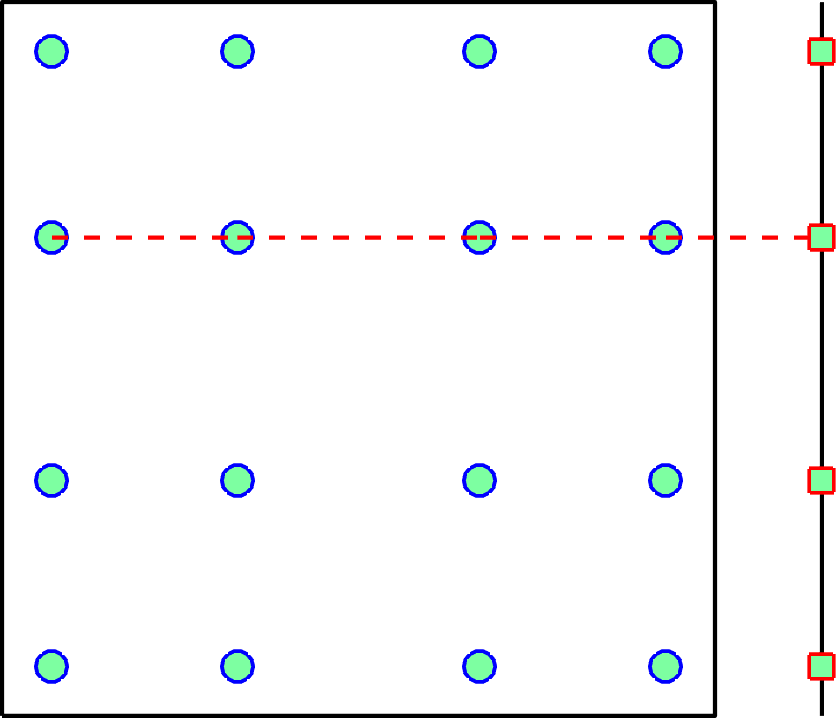
\includegraphics[width=.4\textwidth]{figs/aligned.png}}\label{subfig:aligned}}
\hspace{4em}
\subfloat[Flux evaluations required for non-aligned surface nodes]{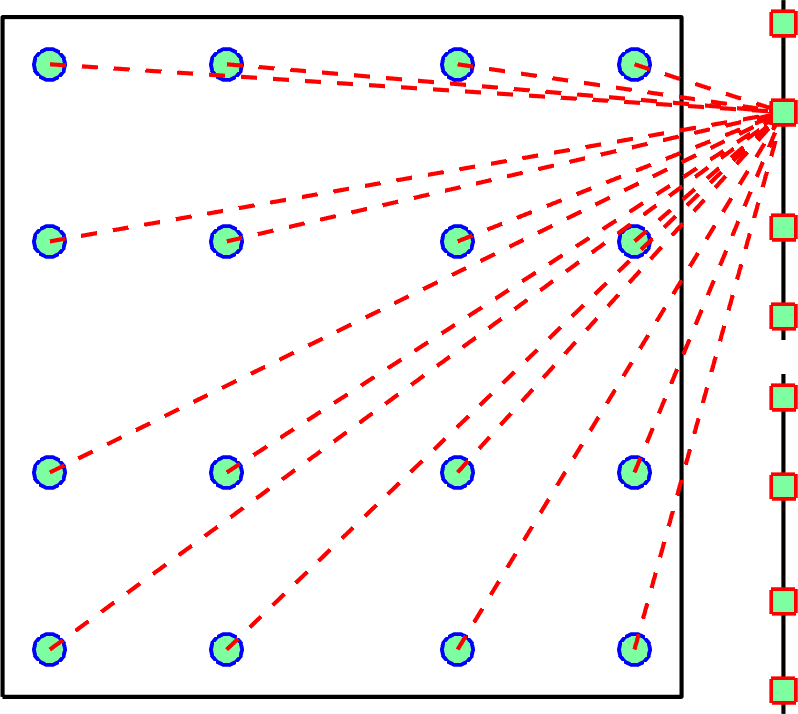
\includegraphics[width=.39\textwidth]{figs/nonaligned.png}\label{subfig:nonaligned}}
\caption{Nodes between which flux evaluations are required for Gauss nodes. Aligned surface nodes (conforming interfaces) require evaluations between each surface node and a line of volume nodes, while non-aligned surface nodes (non-conforming interfaces) require flux evaluations between a surface node and \textit{all} volume nodes.  } %Figure~\ref{subfig:aligned} and \ref{subfig:nonaligned} illustrate when dyadic flux evaluations $\bm{f}^i_S\LRp{\tilde{\bm{u}}_j,\tilde{\bm{u}}_k}$ between nodes are necessary (indicated by dashed red lines) for conforming interfaces (Figure~\ref{subfig:aligned}) and non-conforming interfaces (Figure~\ref{subfig:nonaligned}) under a Gauss collocation scheme.  Conforming interfaces (aligned surface nodes) require evaluations between a surface node and a line of volume nodes, while non-conforming interfaces (nonaligned composite surface nodes) require flux evaluations between a surface node and \textit{all} volume nodes.  The proposed mortar approach (Figure~\ref{subfig:mortar}) reduces the number of dyadic flux evaluations by introducing composite nodes as mortars which couple only to surface nodes. }
\label{fig:fluxsparsity}
\end{figure}

%This work is motivated by complications which arise when designing entropy stable couplings between elements which do not share the same boundary nodes.  This can arise, for example, for hybrid and non-conforming meshes.  
%\paragraph{Hybrid meshes:} entropy stable DG methods on hybrid meshes were introduced in \cite{chan2019skew} using a skew-symmetric formulation.  The resulting methods are stable for more arbitrary choices of surface quadrature, in particular when an SBP property may not hold.  
%
%\paragraph{Non-conforming meshes}

%On conforming meshes, it is most efficient to utilize both Gauss quadrature for volume integrals and Gauss quadrature for face or surface integrals.  For solutions represented in terms of their values at tensor product volume Gauss nodes, extrapolation to face Gauss nodes can be done in an efficient line-by-line manner using one-dimensional interpolation matrices.  
%
%For non-conforming meshes, it can be advantageous to use composite Gauss quadratures on non-conforming interfaces \cite{kozdon2018energy}.  However, interpolating the solution at volume Gauss nodes to split-side Gauss nodes is no longer a one-dimensional operation.  

\section{Entropy stable mortar formulations}
\label{sec:3}

The goal of this work is to reduce computational costs for Gauss collocation schemes in the presence of non-conforming interfaces.  This can be done by treating composite quadrature nodes as a layer of ``mortar'' nodes which are coupled directly to surface nodes, but not directly to the volume nodes, as illustrated in Figure~\ref{fig:gqcon_noncon}.  This results in modifications of the matrices involved in the entropy stable formulation (\ref{eq:esdg}).  These modifications preserve both high order accuracy and entropy stablility, and yield an implementation which is identical to that of (\ref{eq:esdg}) except for a face-local correction to the numerical flux.  
\begin{figure}
\centering
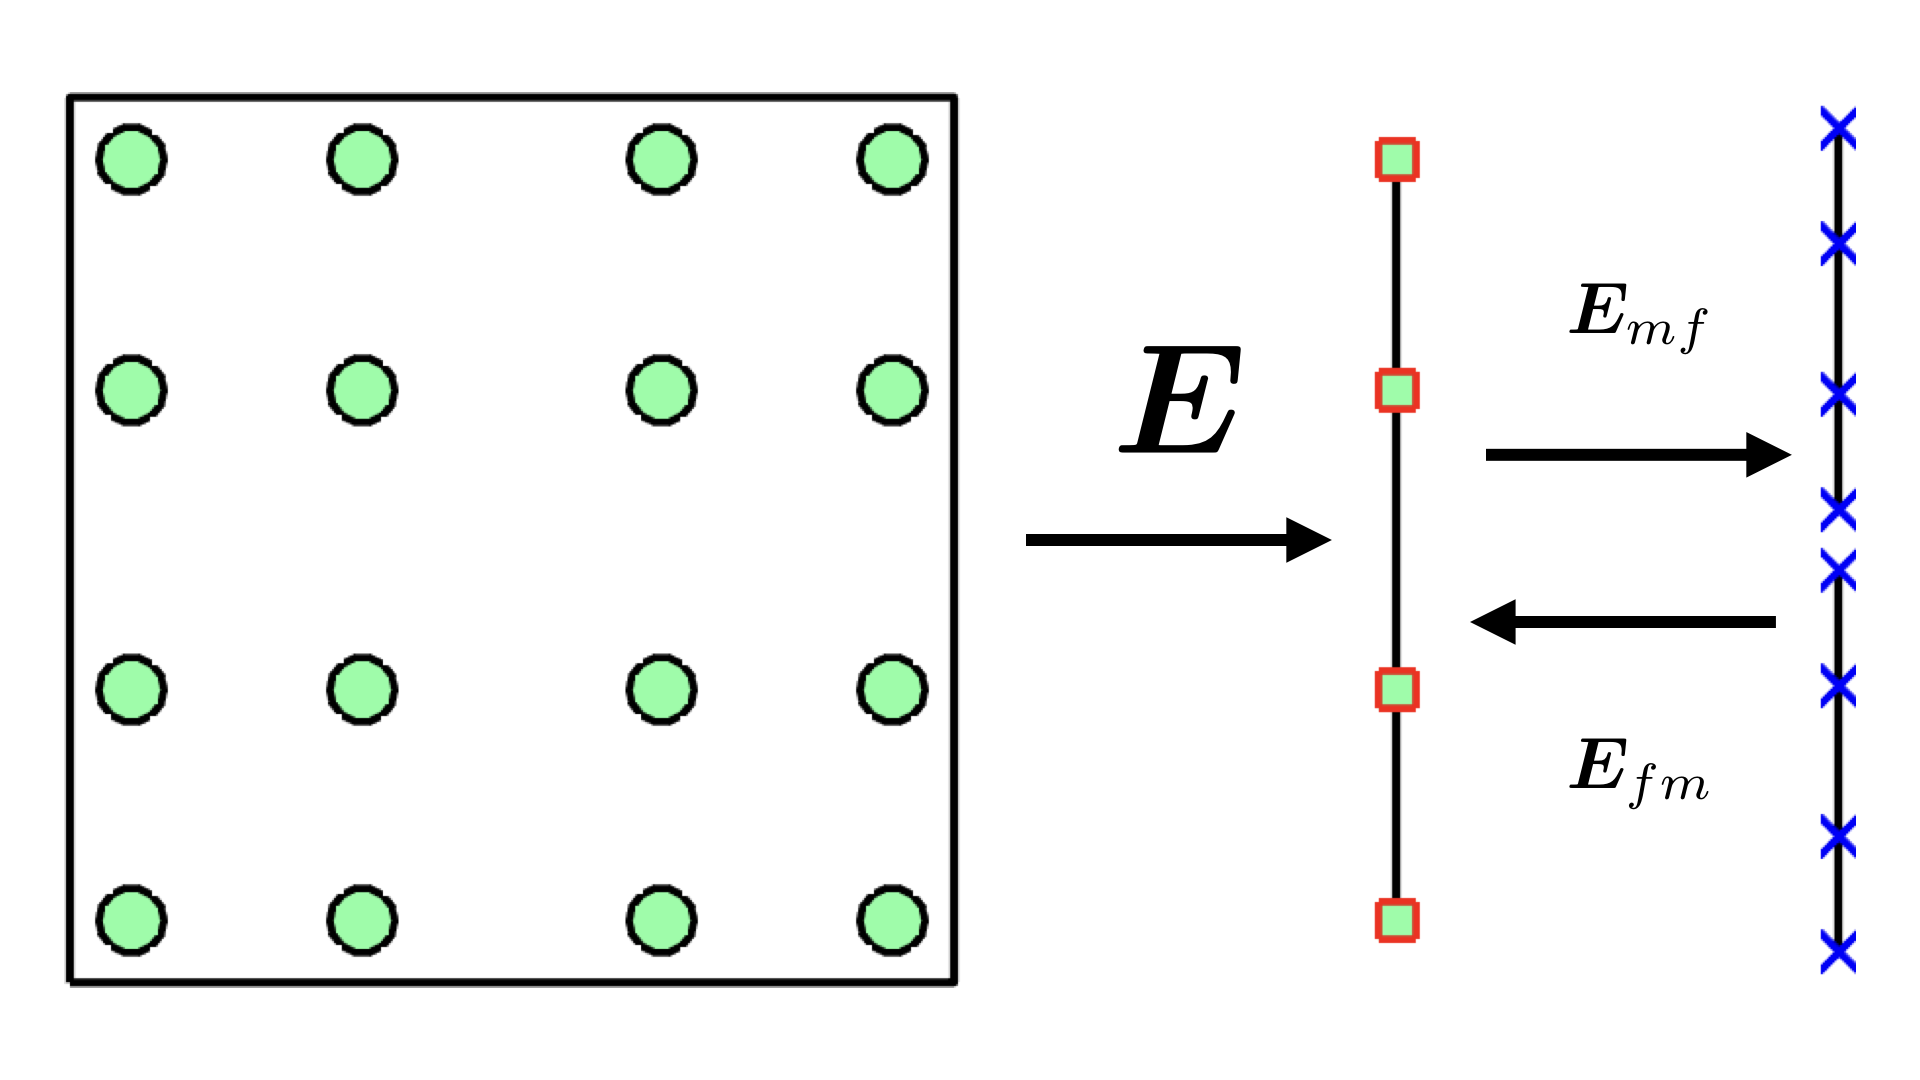
\includegraphics[width=.6\textwidth]{figs/mortar.png}
\caption{Illustration of mortar operators for a Gauss collocation scheme.  The matrix $\bm{E}$ maps from volume quadrature points to surface quadrature points, $\bm{E}_m$ maps from surface to mortar surface points, and $\tilde{\bm{E}}_m$ maps from mortar surface points to surface points. }
\label{fig:gqcon_noncon}
\end{figure}

We introduce new matrices on the reference element $\hat{D}$.  Let $\hat{\bm{x}}$ denote volume collocation points, and let $\hat{\bm{x}}_f$ denote face (surface) points on the boundary $\partial \hat{D}$.  To simplify notation, we assume from this point onwards that the nodes are ordered face-by-face.  In 2D, this implies that $\hat{\bm{x}}_f$ is 
\begin{equation}
\hat{\bm{x}}_f = \begin{bmatrix}
\hat{\bm{x}}_{f,1} &
\hat{\bm{x}}_{f,2} &
\hat{\bm{x}}_{f,3} &
\hat{\bm{x}}_{f,4}
\end{bmatrix}^T,
\label{eq:facenodeordering}
\end{equation}
where $\hat{\bm{x}}_{f,j}$ denotes the vector of 1D nodal positions on the $j$th face of the reference quadrilateral $[-1,1]^2$.  Recall that the matrix $\bm{E}$ as defined in (\ref{eq:EBdefs}) interpolates from volume collocation points $\hat{\bm{x}}$ to surface points $\hat{\bm{x}}_f$; the ordering (\ref{eq:facenodeordering}) simply corresponds to a permutation of the interpolation matrix $\bm{E}$.  

We now introduce a second set of $N_m$ mortar points $\hat{\bm{x}}_m$ on a face of the reference element.  We assume these points also correspond to quadrature nodes with corresponding weights $\bm{w}_m$.  For example, mortar nodes can be composite Gauss or Lobatto quadrature nodes (for $h$ non-conforming interfaces), higher degree Gauss or Lobatto nodes (for $p$ non-conforming interfaces), or identical to the surface nodes $\hat{\bm{x}}_f$ (non-mortar interface).   For simplicity of notation, we assume that each face has the same set of mortar nodes; however, it is straightforward to extend this to the case when the mortar nodes vary face-by-face.  

We define the interpolation matrix $\bm{E}_{mf}$ as the operator which maps values at surface nodes to values at mortar nodes.  In 2D, since the face of a quadrilateral is a 1D line, we can define $\bm{E}_{mf}$ as the block matrix acting on the surface nodes on the four faces 
\[
\bm{E}_{mf} = \bm{I}_{4\times 4}\otimes \bm{E}_m,
\]
where $\bm{I}_{4\times 4}$ is the 4-by-4 identity matrix and $\bm{E}_m$ is the mortar interpolation matrix over the reference face (interval) $[-1,1]$.  The matrix $\bm{E}_m$ is defined in terms of $\hat{x}_{m,i}$, the mortar nodes mapped to the reference interval $[-1,1]$,   
\[
\bm{E}_{mf} = \ell_j(\hat{x}_{m,i}), \qquad 1\leq i \leq N_m, \quad 1\leq j \leq (N+1).
\]
We can define an analogous matrix $\bm{E}_{fm}$ which maps from the mortar nodes back to the surface nodes.  We first define the face mass matrix as the block diagonal matrix whose blocks are 1D diagonal mass matrices
\[
\bm{M}_f = \bm{I}_{4\times 4} \otimes \bm{M}_{\rm 1D}.
\]
These matrices are defined in 2D for simplicity, but are straightforward to extend to 3D.  
The matrix $\bm{E}_{fm}$ can now be defined through a quadrature-based $L^2$ projection 
\[
\bm{E}_{fm} = \bm{M}_f^{-1}\bm{E}_{mf}^T\bm{M}_m, \qquad \bm{M}_m = \bm{I}_{4\times 4}\otimes \diag{\bm{w}_m}.
\]
Finally, we introduce diagonal boundary matrices on surface and mortar nodes 
\begin{equation}
\hat{\bm{B}}_{i,f} = \diag{\hat{\bm{n}}_{i,f}}\bm{M}_f %\circ \bm{w}_f}, 
\qquad \hat{\bm{B}}_{i,m} = \diag{\hat{\bm{n}}_{i,m}}\bm{M}_m,% \circ \bm{w}_m},
\label{eq:Bi}
\end{equation}
where $\hat{\bm{n}}_{i,f}, \hat{\bm{n}}_{i,m}$ are vectors containing components of the scaled reference normals at face and mortar points, respectively.  


Note that $\bm{E}_{fm}$ exactly recovers polynomials of a certain degree on the reference face, where the degree of the polynomial is related to the accuracy of the surface and mortar quadratures.
\begin{lemma}
\label{lemma:Efm}
Suppose the face (surface) quadrature is exact for polynomials of degree $N+N_f$ and mortar quadratures are exact for degree $N+N_m$ polynomials.  Then, $\bm{E}_{fm}$ exactly recovers polynomials of degree $\min(N,N_f,N_m)$.
\end{lemma}
\begin{proof}
Let $u(\bm{x})$ be a polynomial of degree $\min(N,N_f,N_m)$ or less, and let $\bm{u}_f$ be its values on the face (surface) nodes.  Then, $\bm{u}_m = \bm{E}_{mf}\bm{u}_f$ are the interpolated values of the polynomial on the mortar nodes.  Applying $\bm{E}_{fm}$ yields
\[
\bm{E}_{fm}\bm{u}_m = \bm{M}_f^{-1}\bm{E}_{mf}^T\bm{M}_m\bm{E}_{mf}\bm{u}_f.
\]
The entries of $\bm{E}_{mf}^T\bm{M}_m\bm{E}_{mf}$ are integrals of products of Lagrange basis functions with $u(\bm{x})$, where all integrals are approximated using mortar quadrature.  

Since $u$ is degree $\min(N,N_f,N_m)$ and each Lagrange basis function is degree $N$, the integrand is computed exactly under the mortar quadrature.  Moreover, since $u$ is degree $\min(N,N_f,N_m)$, it is also computed exactly using the face (surface) quadrature.  Thus, $\bm{E}_{mf}^T\bm{M}_m\bm{E}_{mf} \bm{u}_f = \bm{M}_f \bm{u}_f$ by exactness of the face and mortar quadratures, and $\bm{E}_{fm}\bm{u}_m = \bm{u}_f$.
\qed\end{proof}

\subsection{Mortar-based hybridized SBP operators}

The matrices $\bm{E}_{mf}, \bm{E}_{fm}, \hat{\bm{B}}_{i,f}, \hat{\bm{B}}_{i,m}$ can now be used to construct SBP operators which involve mortar nodes.  We define the mortar-based hybridized SBP operator on the reference element $\hat{\bm{Q}}_{i,m}$ to be
\begin{align}
\hat{\bm{Q}}_{i,m} = \frac{1}{2}\begin{bmatrix}
\hat{\bm{Q}}_i - \hat{\bm{Q}}_i^T & \bm{E}^T\hat{\bm{B}}_{i,f} & \\
-\hat{\bm{B}}_{i,f}\bm{E} & & \hat{\bm{B}}_{i,f} \bm{E}_{fm}\\
& -\hat{\bm{B}}_{i,m} \bm{E}_{mf} & \hat{\bm{B}}_{i,m}
\end{bmatrix}.
\label{eq:mhsbp}
\end{align}

Since it is not clear at first glance how the hybridized operator $\hat{\bm{Q}}_{i,h}$ or its mortar-based variant $\hat{\bm{Q}}_{i,m}$ can be used to perform differentiation, we review intuitive explanations of each operator.  

Let $\bm{u}$ denote basis coefficients for some function $u(\bm{x})$, and let $f, g$ denote two functions on the reference element.  Suppose $\bm{u}$ satisfies the following matrix system involving the standard hybridized operator $\hat{\bm{Q}}_{i,h}$
\begin{align}
\hat{\bm{M}}\bm{u} = \begin{bmatrix}
\bm{I}\\
\bm{E}
\end{bmatrix}^T \diag{\bm{f}}\hat{\bm{Q}}_{i,h} \diag{\bm{g}}, \qquad \bm{f} = \begin{bmatrix} f(\hat{\bm{x}}) \\ f(\hat{\bm{x}}_f)\end{bmatrix}, \qquad \bm{g} = \begin{bmatrix} g(\hat{\bm{x}}) \\ g(\hat{\bm{x}}_f)\end{bmatrix}.
\label{eq:Qh}
\end{align}
It was shown in \cite{chan2017discretely, chan2019skew} that this corresponds to a high order accurate approximation of $f\pd{g}{x_i}$.  Let $\bm{v}$ denote basis coefficients for some arbitrary degree $N$ polynomial test function.  Expanding out the different blocks of (\ref{eq:Qh}) and using generalized summation by parts for $\hat{\bm{Q}}_i$ yields
\begin{align*}
\hat{\bm{M}}\bm{u} &= 
\diag{f(\hat{\bm{x}})}\hat{\bm{Q}}_i g(\hat{\bm{x}}) + \frac{1}{2}\LRp{\diag{f(\hat{\bm{x}})}\bm{E}^T + \bm{E}^T f(\hat{\bm{x}}_f)}\hat{\bm{B}}_i \LRp{g(\hat{\bm{x}}_f) - \bm{E} g(\hat{\bm{x}})}.
\end{align*}
The latter expression can be interpreted as a boundary correction term.  Since $\bm{E}$ is a high order accurate boundary interpolation operator, this correction term vanishes if $g$ is a degree $N$ polynomial.  
%Replacing quadrature rules by the corresponding integrals, we can re-interpret (\ref{eq:Qh}) as the following variational problem: find a degree $N$ polynomial $u(\bm{x})$ such that, for all polynomials $v(\bm{x})$ of degree $N$,
%\begin{align*}
%\int_{\hat{D}} u(\bm{x}) v(\bm{x}) &= \frac{1}{2} \int_{\hat{D}} \LRp{f\pd{\Pi_N (g)}{x_i}v - g\pd{\Pi_N(fv)}{x_i}} \\
%&+ \frac{1}{2}\int_{\partial \hat{D}} \LRp{g \Pi_N(fv) + \LRp{g - \Pi_N (g)} fv}\hat{n}_i
%\end{align*}
%where $\Pi_N$ denotes the (quadrature-based) $L^2$ projection operator onto degree $N$ polynomials on $\hat{D}$.  Integrating by parts yields
%\begin{align*}
%\int_{\hat{D}} u(\bm{x}) v(\bm{x}) &= \int_{\hat{D}} f\pd{\Pi_N (g)}{x_i}v + \int_{\partial \hat{D}} \LRp{g - \Pi_N(g)}\frac{\LRp{fv+\Pi_N(fv)}}{2}\hat{n}_i
%\end{align*}
%Thus, we can interpret $u(\bm{x})$ as the $L^2$ projection of $f\pd{\Pi_N (g)}{x_i}$ with additional boundary correction terms.  These boundary correction terms vanish if $g$ is a polynomial of degree $N$.  

The mortar-based hybridized SBP operator can be similarly interpreted as a high order differentiation operator.  Recall that $\bm{E}_{mf}$ interpolates from face nodes to mortar nodes, and that $\bm{E}$ interpolates from volume nodes to face nodes.  Thus, the matrix $\bm{E}_{mf}\bm{E}$ interpolates from volume nodes to mortar nodes.  We can use this matrix to replicate (\ref{eq:Qh}) for the mortar-based operator $\hat{\bm{Q}}_{i,m}$.  Let $\bm{u}$ solve the following system
\begin{align}
\hat{\bm{M}}\bm{u} = \begin{bmatrix}
\bm{I}\\
\bm{E}\\
\bm{E}_{mf}\bm{E}
\end{bmatrix}^T \diag{\bm{f}}\hat{\bm{Q}}_{i,m} \diag{\bm{g}}, \qquad \bm{f} = \begin{bmatrix} f(\hat{\bm{x}}) \\ f(\hat{\bm{x}}_f)\\ f(\hat{\bm{x}}_m)\end{bmatrix}, \quad \bm{g} = \begin{bmatrix} g(\hat{\bm{x}}) \\ g(\hat{\bm{x}}_f)\\ g(\hat{\bm{x}}_m)\end{bmatrix}.
\label{eq:Qm}
\end{align}
Expanding out terms yields a similar expression involving multiple correction terms
\begin{align}
\hat{\bm{M}}\bm{u} &= \diag{f(\hat{\bm{x}})}\hat{\bm{Q}}_i{g}(\hat{\bm{x}}) \label{eq:mhsbp_correction}\\
&+ \frac{1}{2} \diag{f(\hat{\bm{x}})}\bm{E}^T\hat{\bm{B}}_{i,f}\LRp{g(\hat{\bm{x}}_f) - \bm{E}g(\hat{\bm{x}})} \nonumber\\
&+ \frac{1}{2} \bm{E}^T\diag{f(\hat{\bm{x}}_f)}\hat{\bm{B}}_{i,f}\LRp{\bm{E}_{fm}g(\hat{\bm{x}}_m) - \bm{E}g(\hat{\bm{x}})} \nonumber\\
&+ \frac{1}{2} \bm{E}^T\bm{E}_{mf}^T\diag{f(\hat{\bm{x}}_m)}\hat{\bm{B}}_{i,m}\LRp{g(\hat{\bm{x}}_m) - \bm{E}_{mf}g(\hat{\bm{x}}_f)} \nonumber
\end{align}
We can show that these correction terms vanish for polynomial functions $g$.  %when $f = 1$ and $g$ is a degree $N$ polynomial.  

\begin{lemma}
Let $f(\bm{x}) = 1$ and suppose that the face (surface) quadrature is exact for polynomials of degree $N+N_f$ and mortar quadratures are exact for degree $N+N_m$ polynomials.  Then, derivative approximations given by the equations (\ref{eq:Qm}) and (\ref{eq:mhsbp_correction}) are exact if $g(\bm{x})$ is a degree $\min(N,N_f,N_m)$ polynomial.
\end{lemma}
\begin{proof}
Following \cite{chan2017discretely}, if $f = 1$  and $g(\bm{x})$ is a degree $N$ polynomial, then  (\ref{eq:mhsbp_correction}) is exact if the correction terms vanish.  The first and third correction terms are zero by the fact that $\bm{E}, \bm{E}_{mf}$ are degree $N$ interpolation operators, and the second correction term vanishes since Lemma~\ref{lemma:Efm} implies that $\bm{E}_{fm}$ exactly recovers polynomials of degree $\min(N,N_f,N_m)$.
\qed\end{proof}

Finally, we note that the mortar-based hybridized SBP operators satisfy a summation by parts property.
\begin{lemma}
\label{lemma:mhsbp}
Let $\hat{\bm{Q}}_{i,m}$ be defined as in (\ref{eq:mhsbp}).  Then, 
\[
\hat{\bm{Q}}_{i,m} + \hat{\bm{Q}}_{i,m}^T = \begin{bmatrix}
\bm{0} && \\
&\bm{0} &\\
&& \hat{\bm{B}}_{i,m}\end{bmatrix}, \qquad \hat{\bm{Q}}_{i,m}\bm{1} = \bm{0}.
\]
\end{lemma}
\begin{proof}
The first property holds if 
\begin{equation}
\hat{\bm{B}}_{i,f} \bm{E}_{fm} = (\hat{\bm{B}}_{i,m} \bm{E}_{mf})^T = \bm{E}_{mf}^T\hat{\bm{B}}_{i,m},  
\label{eq:mhsbpprop}
\end{equation}
where we have used that $\hat{\bm{B}}_{i,m}$ is diagonal.  Recall that $\bm{E}_{fm} = \bm{M}_f^{-1}\bm{E}_{mf}^T\bm{M}_m$.  
Then, by the definition of $\hat{\bm{B}}_{i,m}, \hat{\bm{B}}_{i,h}$ in (\ref{eq:Bi}), we have that
\begin{align*}
\hat{\bm{B}}_{i,f} \bm{E}_{fm} = \diag{\hat{\bm{n}}_{i,f}}\bm{M}_f \bm{M}_f^{-1} \bm{E}_{mf}^T\bm{M}_m 
= \diag{\hat{\bm{n}}_{i,f}} \bm{E}_{mf}^T\bm{M}_m.
\end{align*}
where we have used that $\bm{M}_m$ is diagonal.  Then, since the scaled outward normals $\hat{n}_i$  are constant over each face of the reference element and $\bm{E}_{mf}, \bm{M}_m$ are block matrices (with each block corresponding to a face), we have that
\[
\diag{\hat{\bm{n}}_{i,f}} \bm{E}_{mf}^T\bm{M}_m =\bm{E}_{mf}^T\bm{M}_m \diag{\hat{\bm{n}}_{i,m}}= \bm{E}_{mf}^T\hat{\bm{B}}_{i,m}.
\]  
\qed\end{proof}

%We can now construct an entropy conservative formulation on the reference element using the mortar-based hybridized SBP operator
%\begin{gather}
%\hat{\bm{M}}\td{\bm{u}_h}{t} + \begin{bmatrix} \bm{I} \\ \bm{E} \\ \bm{E}_{mf}\bm{E} \end{bmatrix}^T
%\sum_{i=1}^d \LRp{2\hat{\bm{Q}}_{i,m} \circ \bm{F}_i}\bm{1} + \bm{E}_{mf}^T\hat{\bm{B}}_{i,m}\LRp{\bm{f}_i^*-\bm{f}_i(\tilde{\bm{u}}_m)} = 0 \label{eq:esdgmref}\\
%\tilde{\bm{u}} = \begin{bmatrix}
%\bm{u}_h\\
%\tilde{\bm{u}}_f\\
%\tilde{\bm{u}}_m
%\end{bmatrix}, \qquad \tilde{\bm{u}}_m = \bm{u}\LRp{\bm{E}_{mf}\bm{E}\bm{v}(\bm{u}_h)}%, \qquad \bm{f}^* = \bm{f}_S\LRp{\tilde{\bm{u}}_m^+,\tilde{\bm{u}}_m},
%\end{gather}
%where $\LRp{\bm{F}_i}_{jk} = \bm{f}^i_S\LRp{\tilde{\bm{u}}_j,\tilde{\bm{u}}_k}$ for all indices $j,k$ of $\tilde{\bm{u}}$, and $\bm{f}_i^*$ is a numerical flux used to impose boundary conditions.
%
%\note{Add statement of entropy conservation}


\subsection{Mortar-based formulations on mapped elements}

We can extend the above scheme to mapped curvilinear elements by constructing physical mortar-based hybridized SBP operators in a manner akin to (\ref{eq:curvedQ}).  Abusing notation, we use $\bm{G}_{ij}$ to now denote the vector containing values of $G_{ij} = J\pd{\hat{\bm{x}}_j}{\bm{x}_i}$ at volume, surface, and mortar points.  Then, we define physical operators $\bm{Q}_{i,m}$ via
\begin{equation}
\bm{Q}_{i,m} = \frac{1}{2}\sum_{j=1}^d \diag{\bm{G}_{ij}}\hat{\bm{Q}}_{j,m} + \hat{\bm{Q}}_{j,m} \diag{\bm{G}_{ij}}.
\label{eq:curvedQ_mortar}
\end{equation}
Proofs of entropy conservation (e.g., for the formulation (\ref{eq:esdg})) require that the hybridized SBP operators are conservative (e.g., exact for constants) and satisfy the SBP property.  Entropy conservation for mortar-based formulations on mapped elements will require similar properties.  However, in contrast to hybridized SBP operators, conservation for mapped mortar-based operators requires additional constraints on the accuracy of surface and mortar quadratures relative to the polynomial degree of the geometric mapping.  

We assume now that each geometric mapping from reference element $\hat{D}$ to physical element $D^k$ is a polynomial of degree $N_{\rm geo}$.  We also introduce the space of tensor product polynomials in $d$ dimensions $Q^{N_1,\ldots, N_d}$ as
\[
Q^{N_1,\ldots, N_d} = \LRc{ \hat{x}_1^{i_1}\hat{x}_2^{i_2}\ldots\hat{x}_d^{i_d}, \qquad 0\leq i_k \leq N_k, \quad k = 1,\ldots,d.}
\]
We denote the isotropic tensor product space $Q^N= Q^{N,\ldots,N}$ for conciseness.  

In \cite{chan2019skew}, it was shown that the geometric terms $G_{ij}$ are tensor product polynomials of specific degrees.  For mapped quadrilateral elements, $G_{ij}$ satisfy
\begin{align*}
&G_{i1} \in Q^{N_{\rm geo},N_{\rm geo}-1}\\
&G_{i2} \in Q^{N_{\rm geo}-1,N_{\rm geo}}.
\end{align*}
for $i = 1,2$, and the geometric terms naturally satisfy the GCL condition (\ref{eq:dgcl}).  
%We then have the following lemma:
%\begin{lemma}
%\label{lemma:Qmprops_2d}
%Suppose $D^k$ is a quadrilateral element, and suppose that the surface quadrature is exact for degree ${N+N_f}$ polynomials and mortar quadratures are exact for degree ${N+N_m}$ polynomials.  Then, if $\bm{Q}_{i,m}$ is constructed using (\ref{eq:curvedQ_mortar}) and if $N_{\rm geo} \leq \min(N,N_f+1,N_m+1)$,
%\begin{align*}
%\bm{Q}_{i,m} + \bm{Q}_{i,m}^T &= \bm{B}_{i,m}, \quad \text{(SBP property)}\\
%\bm{Q}_{i,m}\bm{1} &= \bm{0}, \quad \text{(conservation)}.
%\end{align*}
%\end{lemma}
%\begin{proof}
%%The proof mimicks that of Lemma~\ref{lemma:Qhprops}.  
%The SBP property is straightforward to show using the SBP property of $\hat{\bm{Q}}_{i,m}$.  To show conservation, expanding out $\bm{Q}_{i,m}\bm{1} $ yields
%\[
%\bm{Q}_{i,m}\bm{1} = \frac{1}{2}\sum_{j=1}^d \diag{\bm{G}_{ij}}\hat{\bm{Q}}_{j,m}\bm{1} + \hat{\bm{Q}}_{j,m} \diag{\bm{G}_{ij}}\bm{1} = \frac{1}{2}\sum_{j=1}^d\hat{\bm{Q}}_{j,m} \bm{G}_{ij}
%\]
%since $\hat{\bm{Q}}_{j,m}\bm{1} = \bm{0}$ by Lemma~\ref{lemma:mhsbp}.  We can expand out the remaining terms using (\ref{eq:mhsbp_correction}).  However, since $\bm{G}_{ij}$ is constructed by interpolating the values of the polynomial $G_{ij}$, the boundary correction terms in (\ref{eq:mhsbp_correction}) vanish, reducing the expression to 
%\[
%\sum_{j=1}^d\hat{\bm{Q}}_{j,m} \bm{G}_{ij} = \sum_{j=1}^d\hat{\bm{Q}}_{j} G_{ij}(\hat{\bm{x}}) = \bm{0},
%\]
%where $G_{ij}(\hat{\bm{x}})$ denotes the values of the geometric terms at volume nodes $\hat{\bm{x}}$, and the final sum vanishes due to the GCL (\ref{eq:dgcl}) and the fact that $\hat{\bm{Q}}_j$ is exact for degree $N$ polynomials.  
%\qed\end{proof}

For hexahedral elements, it is more challenging to construct geometric terms $G_{ij}$ which satisfy the GCL while retaining high order accuracy.  This is further complicated by the fact that we must take into account the polynomial degrees of $G_{ij}$ when proving conservation for mortar-based SBP operators.  We consider two approaches for computing hexahedral geometric terms in this work:
\begin{enumerate}
\item Approach 1: the construction of $G_{ij}$ from \cite{kopriva2006metric, chan2018efficient}, which yields 
\begin{align*}
&G_{ij} \in Q^{N_{\rm geo}}, \qquad i,j = 1,2,3.
\end{align*}
\item Approach 2: the construction of $G_{ij}$ from \cite{kozdon2018energy} (Appendix C.3), which yields
\begin{align*}
&G_{i1} \in Q^{N_{\rm geo},N_{\rm geo}-1,N_{\rm geo}-1}\\
&G_{i2} \in Q^{N_{\rm geo}-1,N_{\rm geo},N_{\rm geo}-1}\\
&G_{i3} \in Q^{N_{\rm geo}-1,N_{\rm geo}-1,N_{\rm geo}}, \qquad i = 1,2,3.
\end{align*}
\end{enumerate}
These approaches are described in more detail in Appendix~\ref{app:A}.  
\begin{lemma}
\label{lemma:Qmprops_3d}
Suppose $D^k$ is a tensor product element element with tensor product surface quadratures and that $\bm{Q}_{i,m}$ is constructed using (\ref{eq:curvedQ_mortar}).  Suppose also that the surface quadrature is exact for $Q^{N+N_f}$,  the mortar quadrature is exact for $Q^{N+N_m}$.  If 
\begin{enumerate}
\item $D^k$ is a quadrilateral element and $N_{\rm geo} \leq \min(N,N_f+1,N_m+1)$, or
\item $D^k$ is a hexahedral element, $G_{ij}$ is constructed via Approach 1 \cite{kopriva2006metric}, and $N_{\rm geo} \leq \min(N,N_f,N_m)$, or
\item $D^k$ is hexahedral element, $G_{ij}$ is constructed via Approach 2 \cite{kozdon2018energy}, and $N_{\rm geo} \leq \min(N,N_f+1,N_m+1)$, 
\end{enumerate}
then 
\begin{align*}
\bm{Q}_{i,m} + \bm{Q}_{i,m}^T &= \bm{B}_{i,m}, \quad \text{(SBP property)}\\
\bm{Q}_{i,m}\bm{1} &= \bm{0}, \quad \text{(conservation)}.
\end{align*}
\end{lemma}
\begin{proof}
Using the SBP property of $\hat{\bm{Q}}_{i,m}$, proving the SBP property follows the same steps as the proof of Lemma~\ref{lemma:Qhprops}.  To show conservation, expanding out $\bm{Q}_{i,m}\bm{1} $ yields
\[
\bm{Q}_{i,m}\bm{1} = \frac{1}{2}\sum_{j=1}^d \diag{\bm{G}_{ij}}\hat{\bm{Q}}_{j,m}\bm{1} + \hat{\bm{Q}}_{j,m} \diag{\bm{G}_{ij}}\bm{1} = \frac{1}{2}\sum_{j=1}^d\hat{\bm{Q}}_{j,m} \bm{G}_{ij}
\]
since $\hat{\bm{Q}}_{j,m}\bm{1} = \bm{0}$ by Lemma~\ref{lemma:mhsbp}.  Expanding out remaining terms using (\ref{eq:mhsbp_correction}) yields
\begin{align*}
\sum_{j=1}^d \hat{\bm{Q}}_j G_{ij}(\hat{\bm{x}}) &+ \frac{1}{2} \bm{E}^T\hat{\bm{B}}_{j,f}\LRp{G_{ij}(\hat{\bm{x}}_f) - \bm{E}G_{ij}(\hat{\bm{x}})} \\
&+ \frac{1}{2} \bm{E}^T\hat{\bm{B}}_{j,f}\LRp{\bm{E}_{fm}G_{ij}(\hat{\bm{x}}_m) - \bm{E}G_{ij}(\hat{\bm{x}})} \\
&+ \frac{1}{2} \bm{E}^T\bm{E}_{mf}^T\hat{\bm{B}}_{j,m}\LRp{G_{ij}(\hat{\bm{x}}_m) - \bm{E}_{mf}G_{ij}(\hat{\bm{x}}_f)}.
\end{align*}
where $G_{ij}(\hat{\bm{x}}), G_{ij}(\hat{\bm{x}}_f), G_{ij}(\hat{\bm{x}}_m)$ denote the values of $G_{ij}$ at volume, surface, and mortar points.  By the fact that $G_{ij} \in Q^N$ and $\bm{E}, \bm{E}_{mf}$ are degree $N$ interpolation operators, the first and third correction terms vanish.  The remaining boundary correction terms are
\begin{equation}
\bm{E}^T\hat{\bm{B}}_{j,f}\LRp{\bm{E}_{fm}G_{ij}(\hat{\bm{x}}_m) - \bm{E}G_{ij}(\hat{\bm{x}})}.  
\label{eq:bcor}
\end{equation}
Recall that $\hat{\bm{B}}_{i,f}$ is a diagonal matrix whose entries are $\hat{\bm{n}}_{i,m}$ scaled by the mortar quadrature weights.  On tensor product elements, $\hat{\bm{n}}_{i,m}=\pm 1$ on faces where $\hat{x}_i = \pm 1$ and zero otherwise.  Thus, restricting $\hat{x}_1 = \pm 1$ yields the boundary values of $G_{11}$ on faces where the correction term (\ref{eq:bcor}) is non-zero.  We can now show that (\ref{eq:bcor}) vanishes for $i = j = 1$ (the cases of $i = 2,\ldots,d$ are similar).  
\begin{enumerate}
\item If $D^k$ is a quadrilateral element, $G_{11} \in Q^{N_{\rm geo},N_{\rm geo}-1}$, and the surface traces of $G_{11}$ are in the 1D trace space $P^{N_{\rm geo}-1}$.  
\item If $D^k$ is a hexahedral element and $G_{ij}$ is constructed using Approach 1 \cite{kozdon2018energy}, $G_{11} \in Q^{N_{\rm geo}, N_{\rm geo}-1,N_{\rm geo}-1}$, and the surface traces of $G_{11}$ are in the quadrilateral trace space $Q^{N_{\rm geo}-1,N_{\rm geo}-1}$.  
\end{enumerate}
Since $N_{\rm geo} \leq N_m+1$, by Lemma~\ref{lemma:Efm} and assumptions on $N_{\rm geo}, N_f, N_m$, $\bm{E}_{fm}G_{ij}(\hat{\bm{x}}_m) = \bm{E}G_{ij}(\hat{\bm{x}}$ and (\ref{eq:bcor}) vanishes.  

If Approach 1 \cite{kopriva2006metric} is used, then surface traces of $G_{11}$ are contained in $Q^{N_{\rm geo},N_{\rm geo}}$.  Then, (\ref{eq:bcor}) vanishes since $N_{\rm geo} \leq \min(N,N_f,N_m)$.  In both cases, the remaining terms vanish assuming that $G_{ij}$ satisfies the discrete GCL (\ref{eq:dgcl}).
\qed\end{proof}


An entropy conservative mortar-based formulation on mapped elements is then 
\begin{gather}
{\bm{M}}\td{\bm{u}_h}{t} + \begin{bmatrix} \bm{I} \\ \bm{E} \\ \bm{E}_{mf}\bm{E} \end{bmatrix}^T
\sum_{i=1}^d \LRp{2{\bm{Q}}_{i,m} \circ \bm{F}_i}\bm{1} + \bm{E}^T\bm{E}_{mf}^T{\bm{B}}_{i,m}\LRp{\bm{f}_i^*-\bm{f}_i(\tilde{\bm{u}}_m)} = 0 \label{eq:esdgm}\\
\tilde{\bm{u}} = \begin{bmatrix}
\bm{u}_h\\
\tilde{\bm{u}}_f\\
\tilde{\bm{u}}_m
\end{bmatrix}, \qquad \tilde{\bm{u}}_m = \bm{u}\LRp{\bm{E}_{mf}\bm{E}\bm{v}(\bm{u}_h)}, \qquad \bm{f}^* = \bm{f}_S\LRp{\tilde{\bm{u}}_m^+,\tilde{\bm{u}}_m},
\end{gather}
where $\bm{B}_{i,m} = \diag{\bm{n}_{i,m}\circ \bm{w}_m}$ is the diagonal matrix whose entries consist of the scaled physical normals.  Again, we assume geometric terms on curved elements are approximated using polynomials, and that the normals are constructed via (\ref{eq:nJ_Gnhat}) and polynomial interpolation.  


The proof of entropy conservation is algebraically identical to previous proofs, with Lemma~\ref{lemma:Qmprops_3d} used in place of Lemma~\ref{lemma:Qhprops}.




%\note{Note: line DG approach can work, but it's flipped: we increase quadrature strength in the direction \emph{orthogonal} to derivative instead.  May improve accuracy over Lobatto by giving equivalence w/skew form.}


\section{A mortar-based implementation}

While the formulation (\ref{eq:esdgm}) is convenient for analysis, it is less convenient to implement.  However, using properties of the mortar matrices, we can show that the mortar-based formulation (\ref{eq:esdgm}) is equivalent to a conforming formulation (\ref{eq:esdg}) with a modified numerical flux involving face-local correction terms.  

We can reformulate the remaining mortar contributions within (\ref{eq:mortar}).  We decompose $\bm{F}_S$ into interactions between volume nodes, surface nodes, and mortar nodes
\[
\bm{F}_S = \begin{bmatrix}
\bm{F}_S^{vv} & \bm{F}_S^{vf} & \bm{F}_S^{vm}\\
\bm{F}_S^{fv} & \bm{F}_S^{ff} & \bm{F}_S^{fm}\\
\bm{F}_S^{mv} & \bm{F}_S^{mf} & \bm{F}_S^{mm}
\end{bmatrix}
\]
Then, the on-element contributions to (\ref{eq:mortar}) can be expanded as follows
\begin{align*}
&\begin{bmatrix} \bm{I} \\ \bm{E} \\ \bm{E}_m \end{bmatrix}^T
\LRp{\begin{bmatrix}
\bm{Q}_i-\bm{Q}_i^T & \bm{E}^T\bm{B}_i &\\
-\bm{B}_i\bm{E} &  & \bm{B}_{i}{\bm{E}}_m \\
& -\bm{B}_{i,m}{\bm{E}}_m & {\bm{B}}_{i,m}
\end{bmatrix} \circ \bm{F}_S}\bm{1} \\
&= 
\begin{bmatrix} \bm{I}_q \\ \bm{E} \end{bmatrix}^T
\LRp{\begin{bmatrix}
\bm{Q}_i-\bm{Q}_i^T & \bm{E}^T\bm{B}_i\\
-\bm{B}_i\bm{E} & \\
\end{bmatrix} \circ \bm{F}_S}\bm{1} \\
&+ \bm{E}^T \LRp{\bm{B}_i\tilde{\bm{E}}_m\circ \bm{F}_S^{sm}}\bm{1} - \bm{V}_m^T \LRp{ \tilde{\bm{B}}_i\bm{E}_m \circ \bm{F}_S^{ms}}\bm{1}
\end{align*}
Since multiplication by diagonal matrices $\bm{B}_i, \tilde{\bm{B}}_i$ is associative under the Hadamard product, the latter terms can be rewritten as 
\begin{align*}
 \bm{E}^T \LRp{\bm{B}_i\tilde{\bm{E}}_m\circ \bm{F}_S^{sm}}\bm{1} &=  \bm{E}^T \bm{B}_i \LRp{\tilde{\bm{E}}_m\circ \bm{F}_S^{sm}}\bm{1}\\
\bm{V}_m^T \LRp{ \tilde{\bm{B}}_i\bm{E}_m \circ \bm{F}_S^{ms}}\bm{1} &= \bm{V}_m^T \tilde{\bm{B}}_i \LRp{ \bm{E}_m \circ \bm{F}_S^{ms}}\bm{1} = \bm{E}^T \bm{B}_i \tilde{\bm{E}}_m \LRp{ \bm{E}_m \circ \bm{F}_S^{ms}}\bm{1} 
\end{align*}
Then, (\ref{eq:mortar}) can be rewritten as 
\begin{align}
\bm{M}\td{\bm{u}_N}{t} &+ 
\begin{bmatrix} \bm{V}_q \\ \bm{E} \end{bmatrix}^T
\LRp{\begin{bmatrix}
\bm{Q}_i-\bm{Q}_i^T & \bm{E}^T\bm{B}_i\\
-\bm{B}_i\bm{E} & \\
\end{bmatrix} \circ \bm{F}_S}\bm{1} + \bm{E}^T\bm{B}_i \tilde{\bm{f}}^*_i = 0 \label{eq:mortarform}\\
\tilde{\bm{f}}^*_i &= \tilde{\bm{E}}_m\bm{f}^*_i + \LRp{\tilde{\bm{E}}_m\circ \bm{F}_S^{sm}}\bm{1} - \tilde{\bm{E}}_m \LRp{ \bm{E}_m \circ \bm{F}_S^{ms}}\bm{1} 
\nonumber
\end{align}
If the surface and mortar nodes are identical, then 
\[
\bm{E}_m = \tilde{\bm{E}}_m = \bm{I}, \qquad \LRp{\tilde{\bm{E}}_m \circ \bm{F}_S^{sm}}\bm{1} = \LRp{ \bm{E}_m \circ \bm{F}_S^{ms}}\bm{1}
\]
and the correction terms within $\tilde{\bm{f}}^*$ cancel out, and we recover the original scheme from \cite{chan2017discretely}.

Note that in (\ref{eq:mortar2}), the only interactions between surface and mortar nodes occurs within the computation of $\tilde{\bm{f}}^*_i$, which can be done solely on mortar interfaces.  The computational structure of 
\begin{enumerate}
\item Compute volume contributions to the RHS
\item Communicate surface contributions to mortar interfaces and compute $\tilde{\bm{f}}^*_i$.
\item Communicate $\tilde{\bm{f}}^*_i$ back to each element.  
\end{enumerate}

\begin{figure}
\centering
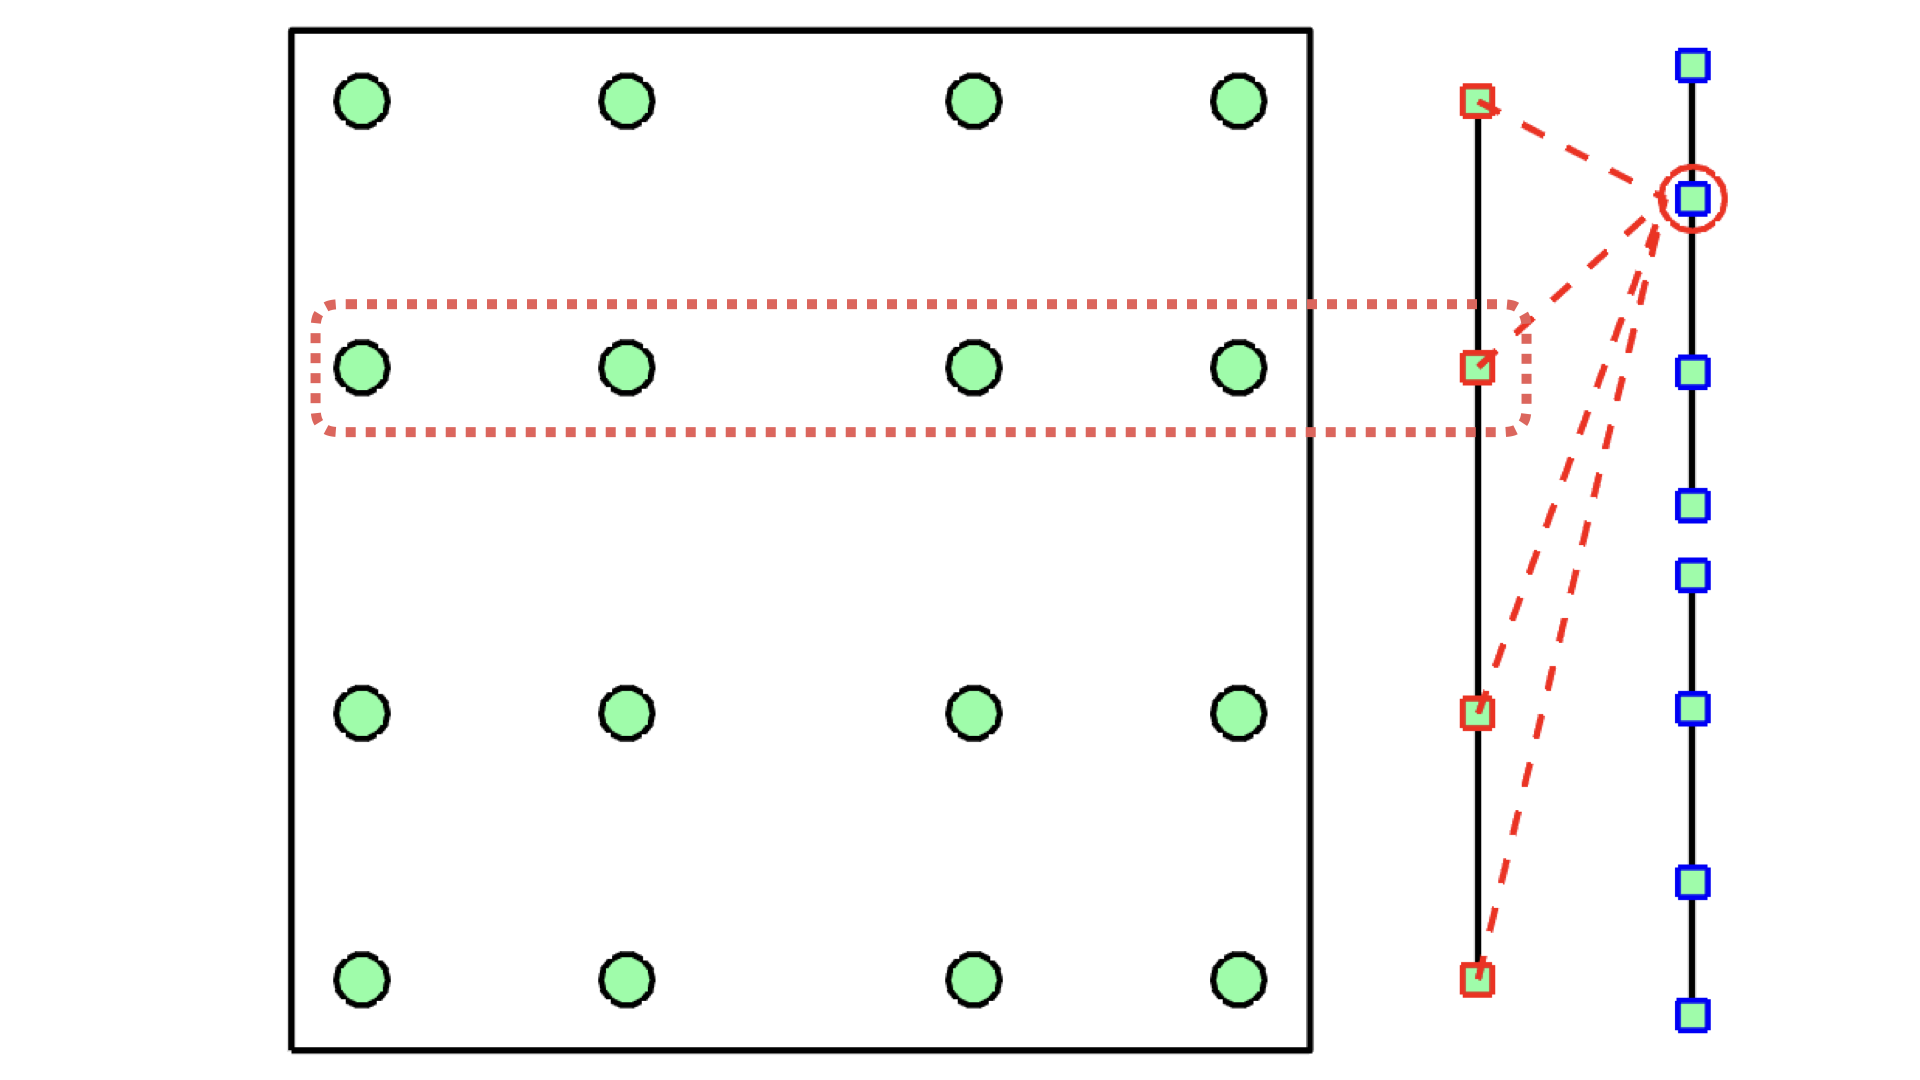
\includegraphics[width=.55\textwidth]{mortar_coupling.png}
\caption{Coupling between volume, surface, and mortar nodes for formulation (\ref{eq:mortarform}).}
\end{figure}


\subsection{Extensions of the mortar-based approach}

\begin{figure}
\centering
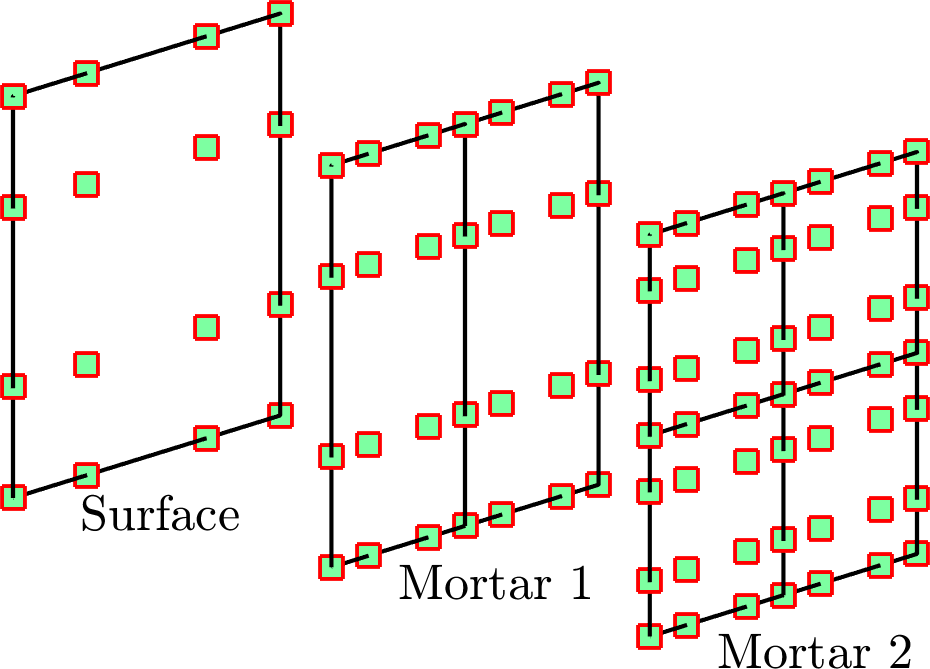
\includegraphics[width=.5\textwidth]{noncon3D.png}
\caption{Two-layer mortars for reduced $O(N^3)$ computational cost on non-conforming hexahedral interfaces.}
\end{figure}

\note{Extensions to 3D meshes: double anisotropic mortar for $O(N^3)$ operations vs $O(N^4)$.}

\note{Extension to $p$ non-conforming meshes is straightforward.  Simply replace the definition of a mortar.}

\note{Extension to general quadratures just requires replacing $\bm{I}$ with $\bm{V}_q, \bm{P}_q$, and redefining $\bm{E}$ matrices.}

\note{Explain why non-hexahedral elements isn't as much of an issue - Shadpey \cite{shadpey2019energy} use this for simplicial elements.  The interpolation operators are dense, and using the mortar-based approach wouldn't actually decrease the number of operations.}



\section{Numerical experiments}


\subsection{2D results}
Figure~\ref{subfig:noncon} shows preliminary results for the 2D compressible Euler equations by the PI on a manually constructed non-conforming quadrilateral mesh, with volume, surface, and mortar quadratures constructed from one-dimensional Lobatto or Gauss quadrature rules.  The PI has verified that this preliminary implementation of the mortar-based formulation is discretely entropy stable.  A preliminary accuracy analysis for the skew-symmetric formulation (\ref{eq:esdgSkew}) also suggests that Lobatto quadrature should achieve an $O(h^N)$ rate of convergence and that Gauss quadrature should achieve an $O(h^{N+1})$ rate of convergence.  Both predicted rates are confirmed in Figure~\ref{subfig:noncon}.

\begin{figure}
\centering
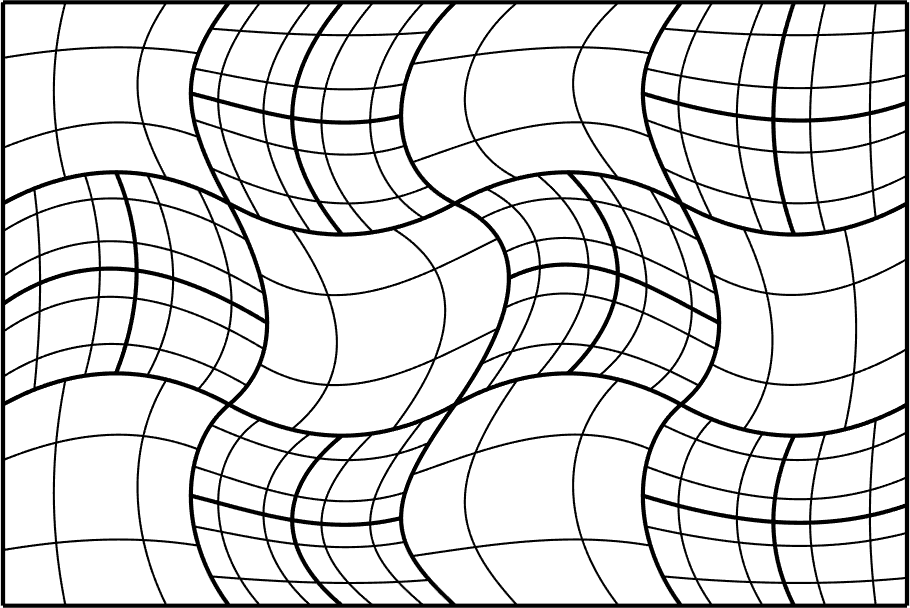
\includegraphics[width=.475\textwidth]{figs/mesh_curved0.png}
\hspace{.5em}
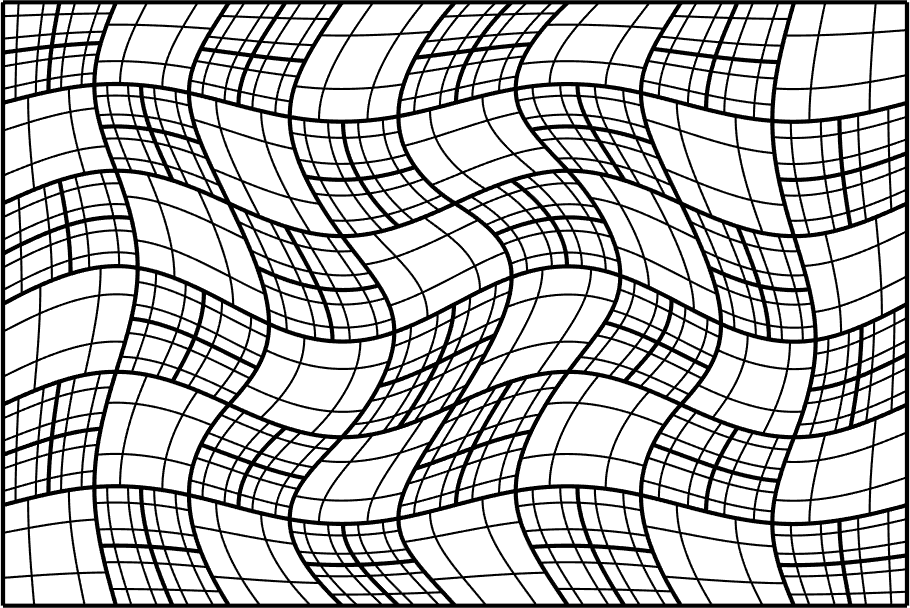
\includegraphics[width=.475\textwidth]{figs/mesh_curved.png}
\caption{Two $N=3$ meshes used in the refinement and entropy conservation studies.}
\end{figure}

\begin{figure}
\centering
%\subfloat[Coarse $N=3$ non-conforming affine mesh]{\raisebox{2.6em}{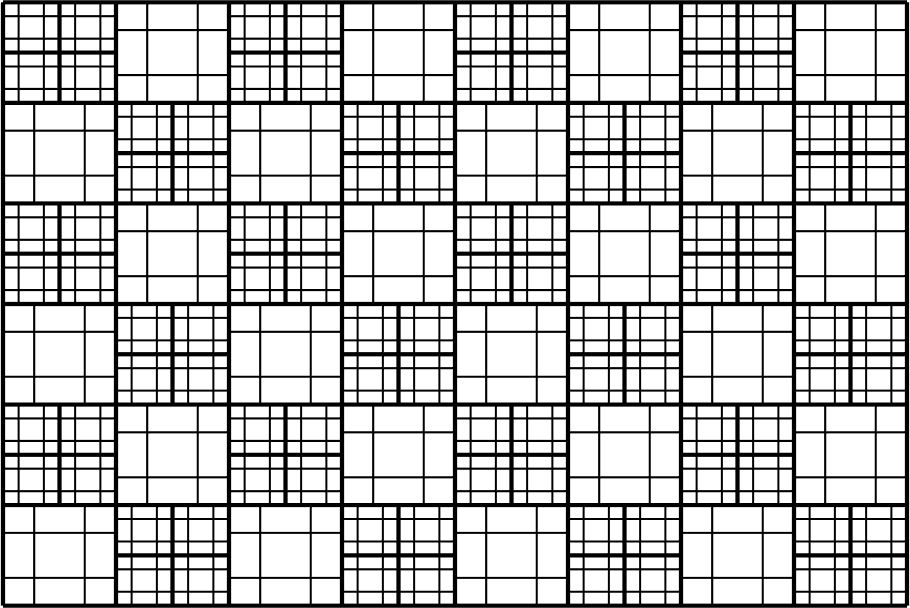
\includegraphics[width=.475\textwidth]{figs/mesh_affine.png}}}
\subfloat[Affine mesh]{
\begin{tikzpicture}
\begin{loglogaxis}[
    width=.49\textwidth,
    xlabel={Mesh size $h$},
    ylabel={$L^2$ errors}, 
    xmax=3.5,
    ymin=1e-4, ymax=5,
    legend pos=south east, legend cell align=left, legend style={font=\tiny},	
    xmajorgrids=true, ymajorgrids=true, grid style=dashed,
    legend entries={Lobatto, Gauss}%, Lobatto-Gauss}    
]
\pgfplotsset{
cycle list={{blue, mark=*}, {red, dashed ,mark=square*}}%,{black, dashdotted ,mark=triangle*}}
}
% N = 1
\addplot+[semithick, mark options={solid, fill=markercolor}]
coordinates{(1.66667,2.78317)(0.833333,2.09894)(0.416667,1.25478)(0.208333,0.490133)};
%\addplot+[semithick, mark options={solid, fill=markercolor}]
%coordinates{(1.66667,2.81566)(0.833333,2.2122)(0.416667,1.44626)(0.208333,0.801638)};
\addplot+[semithick, mark options={solid, fill=markercolor}]
coordinates{(1.66667,2.30772)(0.833333,1.16697)(0.416667,0.303428)(0.208333,0.0576807)};

% N = 2
\addplot+[semithick, mark options={solid, fill=markercolor}]
coordinates{(1.66667,1.51766)(0.833333,0.431437)(0.416667,0.0792017)(0.208333,0.0167253)};
%\addplot+[semithick, mark options={solid, fill=markercolor}]
%coordinates{(1.66667,1.52643)(0.833333,0.436466)(0.416667,0.0801575)(0.208333,0.0167043)};
\addplot+[semithick, mark options={solid, fill=markercolor}]
coordinates{(1.66667,1.06169)(0.833333,0.158534)(0.416667,0.0208737)(0.208333,0.00274974)};

% N = 3
\addplot+[semithick, mark options={solid, fill=markercolor}]
coordinates{(1.66667,0.68797)(0.833333,0.0821894)(0.416667,0.008229)(0.208333,0.000856128)};
%\addplot+[semithick, mark options={solid, fill=markercolor}]
%coordinates{(1.66667,0.685655)(0.833333,0.0815906)(0.416667,0.00838271)(0.208333,0.000889147)};
\addplot+[semithick, mark options={solid, fill=markercolor}]
coordinates{(1.66667,0.455651)(0.833333,0.0328805)(0.416667,0.00233608)(0.208333,0.000143112)};

% N = 4
\addplot+[semithick, mark options={solid, fill=markercolor}]
coordinates{(1.66667,0.242584)(0.833333,0.0170238)(0.416667,0.000922618)};
%\addplot+[semithick, mark options={solid, fill=markercolor}]
%coordinates{(1.66667,0.241312)(0.833333,0.0169965)(0.416667,0.000928106)};
\addplot+[semithick, mark options={solid, fill=markercolor}]
coordinates{(1.66667,0.173237)(0.833333,0.00858261)(0.416667,0.00029501)};

\node at (axis cs:2.4,2.8) {$N = 1$};
\node at (axis cs:2.4,1.3) {$N = 2$};
\node at (axis cs:2.4,.6) {$N = 3$};
\node at (axis cs:2.4,.22) {$N = 4$};
\end{loglogaxis}
\end{tikzpicture}
}
\hspace{.1em}
\subfloat[Curved mesh]{
\begin{tikzpicture}
\begin{loglogaxis}[
    width=.49\textwidth,
    xlabel={Mesh size $h$},
%    ylabel={$L^2$ errors}, 
    xmax=3.5,
    ymin=1e-4, ymax=5,
    legend pos=south east, legend cell align=left, legend style={font=\tiny},	
    xmajorgrids=true, ymajorgrids=true, grid style=dashed,
    legend entries={Lobatto, Gauss}%, Lobatto-Gauss}    
]
\pgfplotsset{
cycle list={{blue, mark=*}, {red, dashed ,mark=square*}}%,{black, dashdotted ,mark=triangle*}}
}
% N = 1
\addplot+[semithick, mark options={solid, fill=markercolor}]
coordinates{(1.66667,2.84018)(0.833333,2.32278)(0.416667,1.44878)(0.208333,0.608642)};
%\addplot+[semithick, mark options={solid, fill=markercolor}]
%coordinates{(1.66667,2.8287)(0.833333,2.36062)(0.416667,1.61841)(0.208333,0.909621)};
\addplot+[semithick, mark options={solid, fill=markercolor}]
coordinates{(1.66667,2.42938)(0.833333,1.40381)(0.416667,0.504184)(0.208333,0.114213)};

% N = 2
\addplot+[semithick, mark options={solid, fill=markercolor}]
coordinates{(1.66667,1.88997)(0.833333,0.710146)(0.416667,0.136728)(0.208333,0.0196411)};
%\addplot+[semithick, mark options={solid, fill=markercolor}]
%coordinates{(1.66667,1.88857)(0.833333,0.709214)(0.416667,0.135323)(0.208333,0.0196621)};
\addplot+[semithick, mark options={solid, fill=markercolor}]
coordinates{(1.66667,1.32118)(0.833333,0.310973)(0.416667,0.0369794)(0.208333,0.00457492)};

% N = 3
\addplot+[semithick, mark options={solid, fill=markercolor}]
coordinates{(1.66667,1.03021)(0.833333,0.211902)(0.416667,0.0195018)(0.208333,0.00184924)};
%\addplot+[semithick, mark options={solid, fill=markercolor}]
%coordinates{(1.66667,1.03557)(0.833333,0.211255)(0.416667,0.0196214)(0.208333,0.0018744)};
\addplot+[semithick, mark options={solid, fill=markercolor}]
coordinates{(1.66667,0.6875)(0.833333,0.0837258)(0.416667,0.0052072)(0.208333,0.000298318)};

% N = 4
\addplot+[semithick, mark options={solid, fill=markercolor}]
coordinates{(1.66667,0.558299)(0.833333,0.0594828)(0.416667,0.00284697)};
%\addplot+[semithick, mark options={solid, fill=markercolor}]
%coordinates{(1.66667,0.557251)(0.833333,0.0593767)(0.416667,0.00284163)};
\addplot+[semithick, mark options={solid, fill=markercolor}]
coordinates{(1.66667,0.330743)(0.833333,0.0204084)(0.416667,0.000691875)};

\node at (axis cs:2.4,3.25) {$N = 1$};
\node at (axis cs:2.4,1.75) {$N = 2$};
\node at (axis cs:2.4,.9) {$N = 3$};
\node at (axis cs:2.4,.425) {$N = 4$};
\end{loglogaxis}
\end{tikzpicture}
}

\caption{Blah}
\end{figure}



\textbf{Gauss Lobatto quadrature}

\textbf{Gauss quadrature}


\subsection{3D results}
\textbf{Gauss Lobatto quadrature}

\textbf{Gauss quadrature}


\appendix

\section{Construction of geometric terms for curved hexahedral elements}
\label{app:A}



\bibliographystyle{unsrt}
\bibliography{refs}


\end{document}


